
\chapter{RESULTADOS}
\label{cap:resultados}

%DESCOMENTAR ESTAS LÍNEAS SI EL CAPÍTULO TIENE FIGURAS O TABLAS
\addtocontents{lof}{{\bf \noindent Figuras del capítulo \arabic{chapter}}}
\addtocontents{lot}{{\bf \noindent Tablas del capítulo \arabic{chapter}}}

En este capítulo se presentan los resultados obtenidos para cada uno de los experimentos. Al igual que en los capítulos donde se describe el diseño del experimento de cada problema, éstos son divididos por problema con el fin de poder realizar la comparación de los resultados entregados por cada uno de los métodos. Los resultados para cada uno de los problemas son presentados por experimento y luego se describe una comparación de éstos. El orden de los experimentos está dado por el caso tradicional de PG y posteriormente el método de islas.

\section{Resultados PM-01}

\subsection{Resultados del proceso evolutivo}

LA GAA aplicada al problema de la mochila bidimensional converge sistemáticamente para diversas ejecuciones realizadas. Este resultado corrobora los resultados previos de la literatura para el mismo problema y otros de optimización combinatoria. La Figura \ref{fig:convergencia_exp1} y la Figura \ref{fig:convergencia_exp2} muestran la convergencia de las distintas ejecuciones de los experimentos 1 y 2 de acuerdo a su \textit{fitness} en el avance de las generaciones, donde cada línea corresponde al mejor algoritmo de cada ejecución del programa para cada uno de los sub-experimentos según corresponda. En esta figura es posible apreciar la rápida convergencia de las ejecuciones y que el \textit{fitness} de cada una de éstas converge a un valor similar. Estos resultados son esperables debido a resultados similares sobre la convergencia en la literatura, además corrobora las consideraciones especificadas en \ref{cap:consideraciones}.

\begingroup
    \centering
    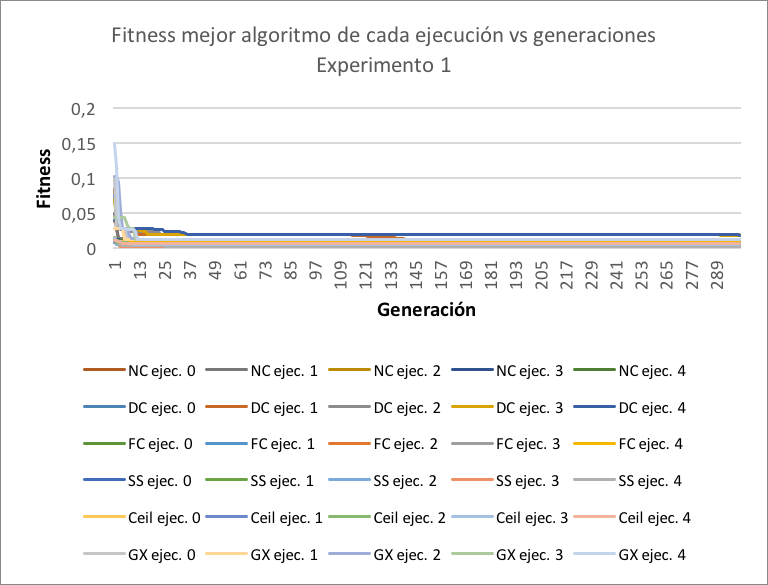
\includegraphics[width=13cm]{images/cap6/convergencia_exp1.png}
    \captionof{figure}{Fitness por generación experimento 1 (Elaboración propia, 2015)}\label{fig:convergencia_exp1}
\endgroup

\begingroup
    \centering
    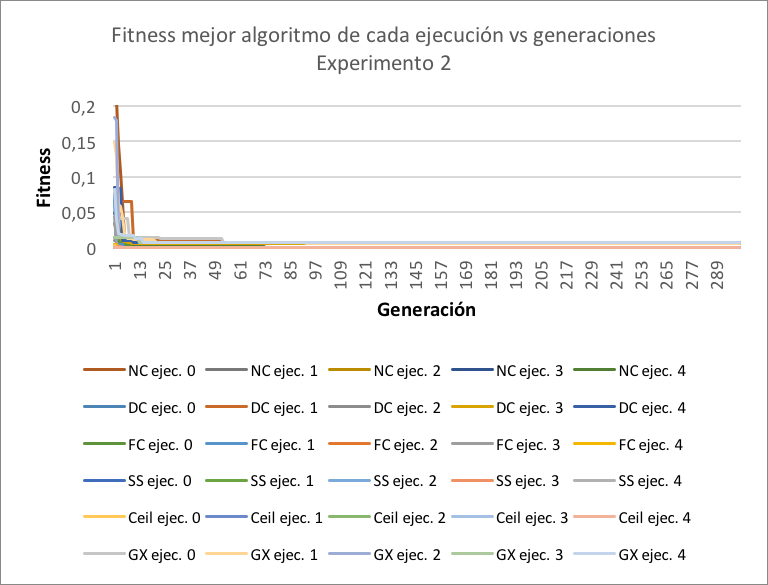
\includegraphics[width=13cm]{images/cap6/convergencia_exp2.png}
    \captionof{figure}{Fitness por generación experimento 2 (Elaboración propia, 2015)}\label{fig:convergencia_exp2}
\endgroup

Existe variedad en relación a la calidad de los algoritmos obtenidos. La distribución de los algoritmos por medio de su calidad en el proceso evolutivo a través de las generaciones es presentada en las Figuras \ref{fig:box_whisker_exp1} y \ref{fig:box_whisker_exp2}. En la Figura \ref{fig:box_whisker_exp1} se presenta el \textit{fitness} de los algoritmos obtenidos en el proceso evolutivo del experimento 1 y ejecución 0 que utiliza el grupo de evolución $SS$ ($ANKPSS1$) y el experimento 2 con ejecución 0 que utiliza el mismo grupo de evolución ($AIKPSS1$), mediante el uso de un gráfico de Box and Whisker. En estas Figuras solo son representadas algunas generaciones ($0, 25, 50, 75, …, 299$), para así poder apreciar la distribución de los algoritmos, debido a su extensa cantidad. Para cada una de las generaciones se presenta una división en cuatro secciones que representan a cada uno de los cuartiles y algunos \textit{outliers}. Cada uno de los cuartiles representa un 25\% (cuartil 1 25\%, cuartil 2 50\%, etc) de los individuos de cada generación. Dentro de las generaciones, aparece una $x$ que representa el promedio de los individuos de la generación, y una línea que divide la “caja” representando la media de los datos. De esta distribución, es posible inferir que el proceso evolutivo, al inicio la mayor cantidad de los individuos posee los peores valores de \textit{fitness}, donde los cuatro cuartiles se encuentran en un rango de $0,6$ a $1,2$ para el experimento 1 y $0,8$ a $1,0$ para el experimento 2, y a medida que avanzan las generaciones, esta distribución tiende a mejores valores. En general, es posible apreciar que existen varios \textit{outliers} en ambos gráficos, los que se encuentran distribuidos en la parte superior de las “cajas”. Esto se debe principalmente a que en cada generación aparecen nuevos individuos auto generados para completar la población, luego de aplicar el proceso de variación (mutación, cruzamiento, reproducción, etc). En ambos gráficos el \textit{fitness} promedio converge a valores menores a $0,2$, mientras que la media tiende a $0$ o valores muy pequeños. De esto último se desprende que al avanzar las generaciones, la mayoría de los individuos, sobre el 50\%, obtienen buenos resultados (menores a $0,1$). La distribución de los demás algoritmos generados por los otros experimentos es similar y puede ser inferida de la Tabla \ref{tab:resumen_exp1} y Tabla \ref{tab:resumen_exp2} donde se muestra el resumen de los experimentos 1 y 2, con sus respectivos sub-experimentos. En estas tablas se muestran datos generales de todos algoritmos obtenidos en la ejecución del sub-experimento para cada uno de los experimentos relacionados al PM-01, por ejemplo “NC ejec. 0” es la ejecución 0 del sub-experimento que utiliza el grupo NC. Dada la gran cantidad de algoritmos generados por sub-experimento y más aún los obtenidos de ambos experimentos durante el proceso evolutivo (aproximadamente 150 mil por sub-experimento), es que se selecciona al mejor de cada ejecución para ser evaluado con las instancias de prueba. Esto resulta en la evaluación de 60 algoritmos, siendo cinco los extraídos de cada uno de los 12 experimentos (experimento 1a, experimento 2a, experimento 1b, experimento 2b, etc). Los algoritmos a evaluar son los propuestos en la Tabla \ref{tab:mejores_pm01_exp1} y Tabla \ref{tab:mejores_pm01_exp2} para los experimentos 1 y 2 respectivamente. En las tablas donde se presentan los mejores algoritmos, el nombre que éstos tienen posee la siguiente forma: Algoritmo - Experimento (Tradicional \textbf{(N)} o co-evolución utilizando método de islas \textbf{(I)}) - Problema - Grupo instancias - Correlativo de 1 a 5. Un ejemplo de esto último es ANKPNC1, que se lee como Algoritmo (A) del experimento tradicional (N) para el problema de la mochila (KP) utilizando el grupo de instancias NC (NC) obtenido en la ejecución 1.

\begingroup
    \centering
    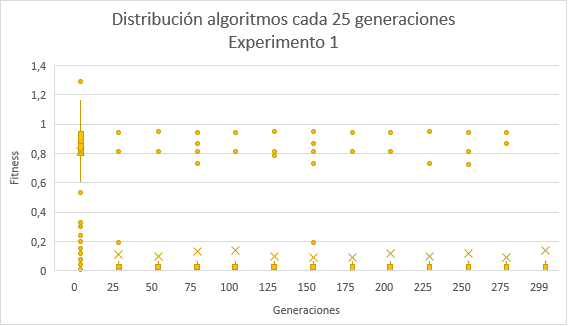
\includegraphics[width=13cm]{images/cap6/box_whisker_exp1.png}
    \captionof{figure}{Distribución algoritmos experimento 1 (Elaboración propia, 2015)}\label{fig:box_whisker_exp1}
\endgroup

\begingroup
    \centering
    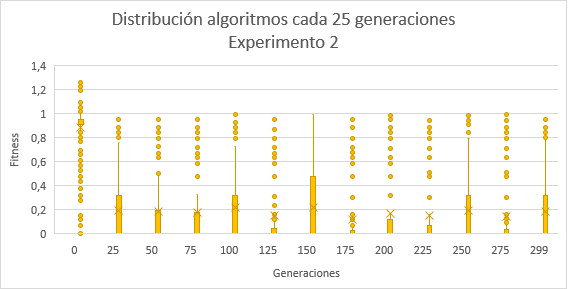
\includegraphics[width=13cm]{images/cap6/box_whisker_exp2.png}
    \captionof{figure}{Distribución algoritmos experimento 2 (Elaboración propia, 2015)}\label{fig:box_whisker_exp2}
\endgroup

\begin{table}[hbtp!]
\caption{Datos generales de los algoritmos obtenidos en el experimento 1}\label{tab:resumen_exp1}
\small
\centering
\begin{center}
\rowcolors{2}{gray!25}{white}
\begin{tabular}{c|ccc|ccc|ccc}
\hline
{\textbf{}} & \multicolumn{3}{c}{{\textbf{Fitness}}} & \multicolumn{3}{c}{{\textbf{Nº Nodos}}} & \multicolumn{3}{c}{{\textbf{Altura}}} \\ \hline
{\textbf{Nombre}} & \textbf{Peor} &	\textbf{Prom.} & \textbf{Mejor} & \textbf{Min.} & \textbf{Prom.} & \textbf{Máximo} & \textbf{Min.} & \textbf{Prom.} & \textbf{Máximo} \\ \hline
NC ejec. 0 & 1,1688 & 0,2232 & 0,0038 & 2 & 13,08 & 122 & 2 & 5,27 & 10 \\
NC ejec. 1 & 1,2133 & 0,2827 & 0,0037 & 2 & 12,16 & 116 & 2 & 4,70 & 10 \\
NC ejec. 2 & 1,3316 & 0,2309 & 0,0039 & 2 & 12,13 & 133 & 2 & 5,89 & 10 \\
NC ejec. 3 & 1,1607 & 0,2365 & 0,0057 & 2 & 10,59 & 121 & 2 & 4,38 & 10 \\
NC ejec. 4 & 1,2449 & 0,1393 & 0,0047 & 2 & 10,48 & 138 & 2 & 4,45 & 10 \\ \hline
DC ejec. 0 & 1,1567 & 0,2557 & 0,0178 & 2 & 12,52 & 109 & 2 & 5,78 & 10 \\
DC ejec. 1 & 1,1516 & 0,2262 & 0,0118 & 2 & 12,89 & 139 & 2 & 5,23 & 10 \\
DC ejec. 2 & 1,3174 & 0,2372 & 0,0187 & 2 & 12,39 & 126 & 2 & 4,60 & 10 \\
DC ejec. 3 & 1,2252 & 0,2168 & 0,0176 & 2 & 11,65 & 109 & 2 & 5,01 & 10 \\
DC ejec. 4 & 1,1508 & 0,2276 & 0,0178 & 2 & 10,81 & 144 & 2 & 5,40 & 10 \\ \hline
FC ejec. 0 & 1,1567 & 0,1775 & 0,0093 & 2 & 11,49 & 98 & 2 & 4,18 & 10 \\
FC ejec. 1 & 1,2166 & 0,1215 & 0,0096 & 2 & 6,54 & 105 & 2 & 3,56 & 10 \\
FC ejec. 2 & 1,2905 & 0,1699 & 0,0080 & 2 & 11,44 & 124 & 2 & 4,25 & 10 \\
FC ejec. 3 & 1,2133 & 0,2404 & 0,0078 & 2 & 9,47 & 103 & 2 & 4,93 & 10 \\
FC ejec. 4 & 1,2000 & 0,1936 & 0,0096 & 2 & 7,04 & 106 & 2 & 3,25 & 10 \\ \hline
SS ejec. 0 & 1,2900 & 0,1289 & 0,0021 & 2 & 10,85 & 123 & 2 & 3,96 & 10 \\
SS ejec. 1 & 1,3033 & 0,0420 & 0,0021 & 2 & 11,00 & 121 & 2 & 4,42 & 10 \\
SS ejec. 2 & 1,2389 & 0,2545 & 0,0021 & 2 & 11,27 & 108 & 2 & 4,76 & 10 \\
SS ejec. 3 & 1,2067 & 0,1964 & 0,0022 & 2 & 8,50 & 131 & 2 & 4,36 & 10 \\
SS ejec. 4 & 1,2493 & 0,1792 & 0,0021 & 2 & 10,42 & 125 & 2 & 5,43 & 10 \\ \hline
Ceil ejec. 0 & 1,2383 & 0,2175 & 0,0051 & 2 & 12,36 & 132 & 2 & 4,24 & 10 \\
Ceil ejec. 1 & 1,1510 & 0,1895 & 0,0058 & 2 & 11,05 & 117 & 2 & 5,35 & 10 \\
Ceil ejec. 2 & 1,2293 & 0,1332 & 0,0048 & 2 & 12,75 & 136 & 2 & 5,88 & 10 \\
Ceil ejec. 3 & 1,2128 & 0,1866 & 0,0048 & 2 & 10,51 & 134 & 2 & 4,26 & 10 \\
Ceil ejec. 4 & 1,2338 & 0,2189 & 0,0057 & 2 & 8,65 & 124 & 2 & 4,38 & 10 \\ \hline
GX ejec. 0 & 1,2172 & 0,2187 & 0,0126 & 2 & 8,86 & 120 & 2 & 4,60 & 10 \\
GX ejec. 1 & 1,1209 & 0,1530 & 0,0126 & 2 & 10,56 & 102 & 2 & 4,53 & 10 \\
GX ejec. 2 & 1,3110 & 0,2769 & 0,0123 & 2 & 12,16 & 139 & 2 & 4,68 & 10 \\
GX ejec. 3 & 1,1931 & 0,2250 & 0,0126 & 2 & 8,40 & 115 & 2 & 4,36 & 10 \\
GX ejec. 4 & 1,1819 & 0,2192 & 0,0126 & 2 & 9,37 & 123 & 2 & 4,43 & 10 \\
\hline
\end{tabular}
\end{center}
\caption*{(Elaboración propia, 2015)}
\end{table}

\begin{table}[hbtp!]
\caption{Datos generales de los algoritmos obtenidos en el experimento 2}\label{tab:resumen_exp2}
\small
\centering
\begin{center}
\rowcolors{2}{gray!25}{white}
\begin{tabular}{c|ccc|ccc|ccc}
\hline
{\textbf{}} & \multicolumn{3}{c}{{\textbf{Fitness}}} & \multicolumn{3}{c}{{\textbf{Nº Nodos}}} & \multicolumn{3}{c}{{\textbf{Altura}}} \\ \hline
{\textbf{Nombre}} & \textbf{Peor} &	\textbf{Prom.} & \textbf{Mejor} & \textbf{Min.} & \textbf{Prom.} & \textbf{Máximo} & \textbf{Min.} & \textbf{Prom.} & \textbf{Máximo} \\ \hline
NC ejec. 0 & 1,2700 & 0,2838 & 0,0000 & 2 & 9,67 & 120 & 2 & 4,89 & 10 \\
NC ejec. 1 & 1,3033 & 0,3810 & 0,0000 & 2 & 10,50 & 163 & 2 & 4,96 & 10 \\
NC ejec. 2 & 1,3233 & 0,3724 & 0,0000 & 2 & 10,42 & 127 & 2 & 4,28 & 10 \\
NC ejec. 3 & 1,3200 & 0,3549 & 0,0000 & 2 & 10,29 & 129 & 2 & 5,00 & 10 \\
NC ejec. 4 & 1,3000 & 0,3109 & 0,0000 & 2 & 7,67 & 133 & 2 & 4,06 & 10 \\ \hline
DC ejec. 0 & 1,2033 & 0,4185 & 0,0057 & 2 & 9,07 & 96 & 2 & 4,22 & 10 \\
DC ejec. 1 & 1,2967 & 0,3334 & 0,0057 & 2 & 9,97 & 119 & 2 & 4,15 & 10 \\
DC ejec. 2 & 1,2700 & 0,4415 & 0,0056 & 2 & 12,35 & 120 & 2 & 4,13 & 10 \\
DC ejec. 3 & 1,2667 & 0,3839 & 0,0057 & 2 & 9,74 & 110 & 2 & 4,63 & 10 \\
DC ejec. 4 & 1,2700 & 0,3774 & 0,0069 & 2 & 9,34 & 111 & 2 & 3,73 & 10 \\ \hline
FC ejec. 0 & 1,3733 & 0,3392 & 0,0000 & 2 & 8,27 & 142 & 2 & 4,08 & 10 \\
FC ejec. 1 & 1,2733 & 0,3799 & 0,0000 & 2 & 7,35 & 138 & 2 & 3,96 & 10 \\
FC ejec. 2 & 1,2803 & 0,3511 & 0,0000 & 2 & 8,94 & 140 & 2 & 4,23 & 10 \\
FC ejec. 3 & 1,2333 & 0,3418 & 0,0000 & 2 & 7,26 & 112 & 2 & 3,70 & 10 \\
FC ejec. 4 & 1,2267 & 0,2614 & 0,0000 & 2 & 6,31 & 100 & 2 & 3,51 & 10 \\ \hline
SS ejec. 0 & 1,2600 & 0,1862 & 0,0000 & 2 & 11,24 & 108 & 2 & 4,86 & 10 \\
SS ejec. 1 & 1,2267 & 0,2571 & 0,0000 & 2 & 9,27 & 98 & 2 & 4,15 & 10 \\
SS ejec. 2 & 1,3100 & 0,2828 & 0,0000 & 2 & 10,86 & 123 & 2 & 3,95 & 10 \\
SS ejec. 3 & 1,1867 & 0,2619 & 0,0000 & 2 & 10,96 & 130 & 2 & 4,78 & 10 \\
SS ejec. 4 & 1,3167 & 0,2163 & 0,0000 & 2 & 10,85 & 125 & 2 & 4,46 & 10 \\ \hline
Ceil ejec. 0 & 1,2267 & 0,2381 & 0,0000 & 2 & 9,14 & 107 & 2 & 4,32 & 10 \\
Ceil ejec. 1 & 1,2400 & 0,2326 & 0,0000 & 2 & 9,37 & 119 & 2 & 4,65 & 10 \\
Ceil ejec. 2 & 1,2733 & 0,1516 & 0,0000 & 2 & 9,38 & 118 & 2 & 4,27 & 10 \\
Ceil ejec. 3 & 1,3067 & 0,2221 & 0,0000 & 2 & 9,84 & 122 & 2 & 4,36 & 10 \\
Ceil ejec. 4 & 1,2408 & 0,2770 & 0,0000 & 2 & 9,42 & 115 & 2 & 4,35 & 10 \\ \hline
GX ejec. 0 & 1,2900 & 0,3662 & 0,0075 & 2 & 9,27 & 120 & 2 & 4,35 & 10 \\
GX ejec. 1 & 1,2567 & 0,3916 & 0,0064 & 2 & 11,46 & 133 & 2 & 4,61 & 10 \\
GX ejec. 2 & 1,2667 & 0,3458 & 0,0077 & 2 & 10,79 & 110 & 2 & 4,63 & 10 \\
GX ejec. 3 & 1,2932 & 0,3675 & 0,0075 & 2 & 9,65 & 123 & 2 & 4,67 & 10 \\
GX ejec. 4 & 1,2933 & 0,3994 & 0,0076 & 2 & 10,44 & 122 & 2 & 5,17 & 10 \\
\hline
\end{tabular}
\end{center}
\caption*{(Elaboración propia, 2015)}
\end{table}

En relación al \textit{fitness}, no existe una gran variación en la calidad de la GAA para los distintos algoritmos obtenidos durante el proceso evolutivo para el mismo conjunto de instancias. En las tablas \ref{tab:resumen_exp1} y \ref{tab:resumen_exp2} aparecen datos del mejor, peor y promedio del \textit{fitness} de todos los algoritmos generados utilizando alguno de los grupos de instancias clasificados en el sub-capítulo \ref{cap:sel_casos_adapt_pm01}. En relación a la Tabla \ref{tab:resumen_exp1}, es posible apreciar que el resultado tanto del mejor, peor y el promedio del \textit{fitness} de los algoritmos tiende a valores similares, lo que complementa las consideraciones mencionadas en \ref{cap:consideraciones}. En relación a los resultados del \textit{fitness} obtenido entre los distintos grupos de instancias, es posible apreciar que en algunos casos, existe una mayor diferencia que la presentada en los resultados dentro del mismo grupo, lo que se debe principalmente a las características del grupo de instancias utilizado en el proceso evolutivo. Para la Tabla \ref{tab:resumen_exp2} se ve que ocurre un efecto similar, tanto en la relación entre los algoritmos del mismo grupo, como en la comparación con los de otros grupos. Finalmente, los resultados que se obtienen en cada uno de los grupos al ser comparados entre experimentos, presentan una variación en la que los algoritmos del experimento 1 obtienen mejores resultados. Esta variación ocurre por que en el experimento 2 se generan algoritmos en distintas poblaciones con distintos criterios de evaluación (islas), lo que conlleva a una mayor variabilidad que la presentada en el experimento 1.

La variación de los algoritmos obtenidos en la GAA está relacionada con la estructura  que posee el árbol sintáctico obtenido durante el proceso evolutivo. En las tablas \ref{tab:resumen_exp1} y \ref{tab:resumen_exp2} aparecen datos del máximo, mínimo y promedio del número de nodos y la altura. Con respecto al número de nodos, existe variación en los algoritmos del mismo grupo y al ser comparados entre los distintos grupos. Aunque el número máximo de nodos alcanza valores sobre 100, el promedio es siempre menor a 15, cuyo valor fue determinado como máximo para no interferir en la calidad de los algoritmos (factor de legibilidad, véase \ref{cap:func_eval_pm01}). En relación a la altura de los árboles que representan a los algoritmos, se ve que también existe variación tanto entre los grupos como al compararlos con otros. El promedio de éstos tiende a valores entre 3 y 5, lo que se relaciona directamente con el número máximo permitido de nodos, ya que algunos de estos nodos representan funciones, las que solo tienen permitido un número determinado de hijos.

La calidad de los algoritmos obtenidos mediante el proceso evolutivo no tiene relación con el tiempo que demora el proceso evolutivo ni la generación en la que el o los mejores algoritmos aparecen dentro de la ejecución de este proceso. En las tablas \ref{tab:mejores_pm01_exp1} y \ref{tab:mejores_pm01_exp2}, es posible apreciar el tiempo de evolución de cada una de las ejecuciones y la generación en la que aparece el mejor individuo de ésta. En estas tablas es posible notar que existe variación tanto en el tiempo de cada una de las ejecuciones del proceso evolutivo y en la generación en la que el mejor individuo aparece.

El tamaño de los árboles que componen los algoritmos obedece al rango de tamaño predefinido en la función de legibilidad que se encuentra dentro de la función de evaluación (\textit{fitness}). En la Tabla \ref{tab:mejores_pm01_exp1} y \ref{tab:mejores_pm01_exp2} se muestra que no existe una convergencia hacia árboles de similares dimensiones. Como se observa en estas tablas, los árboles seleccionados varían entre 3 y 15 nodos con una altura entre 2 y 7 para el experimento 1, y entre 3 y 15 nodos, con una altura entre 2 y 6 para el experimento 2.

\begin{table}[hbtp!]
\caption{Datos generales del mejor algoritmo de cada experimento del experimento 1}\label{tab:mejores_pm01_exp1}
\small
\centering
\begin{center}
\rowcolors{2}{gray!25}{white}
\begin{tabular}{cccccc}
{\textbf{{Nombre}}} & {\textbf{{Fitness}}} & {\textbf{\begin{tabular}[c]{@{}c@{}}Nº de \\nodos\end{tabular}}} & {\textbf{{Altura}}} & {\textbf{\begin{tabular}[c]{@{}c@{}}Ejecución en la \\que aparece\end{tabular}}} & {\textbf{\begin{tabular}[c]{@{}c@{}}Tiempo \\(min)\end{tabular}}}\\ \hline
ANKPNC1 & 0,0038 & 15 & 6 & 30 & 21,10 \\
ANKPNC2 & 0,0037 & 15 & 5 & 231 & 23,09 \\
ANKPNC3 & 0,0039 & 14 & 7 & 100 & 24,40 \\
ANKPNC4 & 0,0057 & 15 & 5 & 14 & 19,25 \\
ANKPNC5 & 0,0047 & 9 & 4 & 17 & 18,58 \\ \hline
ANKPDC1 & 0,0187 & 14 & 6 & 291 & 17,16 \\
ANKPDC2 & 0,0118 & 15 & 6 & 138 & 30,04 \\
ANKPDC3 & 0,0187 & 15 & 5 & 57 & 19,65 \\
ANKPDC4 & 0,0187 & 13 & 5 & 16 & 17,30 \\
ANKPDC5 & 0,0187 & 15 & 7 & 148 & 19,49 \\ \hline
ANKPFC1 & 0,0093 & 14 & 4 & 4 & 17,63 \\
ANKPFC2 & 0,0096 & 3 & 2 & 0 & 22,49 \\
ANKPFC3 & 0,0082 & 14 & 5 & 129 & 22,33 \\
ANKPFC4 & 0,0078 & 15 & 8 & 282 & 24,55 \\
ANKPFC5 & 0,0096 & 3 & 2 & 0 & 19,92 \\ \hline
ANKPSS1 & 0,0021 & 14 & 4 & 4 & 13,65 \\
ANKPSS2 & 0,0021 & 10 & 4 & 3 & 19,70 \\
ANKPSS3 & 0,0021 & 15 & 5 & 94 & 20,74 \\
ANKPSS4 & 0,0022 & 5 & 3 & 3 & 18,90 \\
ANKPSS5 & 0,0021 & 9 & 5 & 32 & 16,88 \\ \hline
ANKPCeil1 & 0,0051 & 13 & 4 & 23 & 10,15 \\
ANKPCeil2 & 0,0058 & 13 & 5 & 12 & 10,96 \\
ANKPCeil3 & 0,0049 & 15 & 7 & 95 & 14,78 \\
ANKPCeil4 & 0,0048 & 11 & 4 & 8 & 11,63 \\
ANKPCeil5 & 0,0068 & 5 & 3 & 36 & 12,61 \\ \hline
ANKPGX1 & 0,0167 & 8 & 5 & 8 & 13,45 \\
ANKPGX2 & 0,0073 & 8 & 5 & 5 & 11,66 \\
ANKPGX3 & 0,0164 & 9 & 4 & 46 & 13,23 \\
ANKPGX4 & 0,0077 & 9 & 4 & 10 & 14,42 \\
ANKPGX5 & 0,0142 & 15 & 5 & 11 & 12,46 \\
\hline
\end{tabular}
\end{center}
\caption*{(Elaboración propia, 2015)}
\end{table}

\begin{table}[hbtp!]
\caption{Datos generales del mejor algoritmo de cada experimento del experimento 2}\label{tab:mejores_pm01_exp2}
\small
\centering
\begin{center}
\rowcolors{2}{gray!25}{white}
\begin{tabular}{ccccccc}
{\textbf{{Nombre}}} & {\textbf{{Fitness}}} & {\textbf{\begin{tabular}[c]{@{}c@{}}Nº de \\nodos\end{tabular}}} & {\textbf{{Altura}}} & {\textbf{\begin{tabular}[c]{@{}c@{}}Ejecución en la \\que aparece\end{tabular}}} & {\textbf{\begin{tabular}[c]{@{}c@{}}Isla en la \\que aparece\end{tabular}}} & {\textbf{\begin{tabular}[c]{@{}c@{}}Tiempo \\(min)\end{tabular}}}\\ \hline
AIKPNC1 & 0,0048 & 13 & 6 & 2 & 23 & 22,66 \\
AIKPNC2 & 0,0047 & 11 & 5 & 2 & 112 & 26,93 \\
AIKPNC3 & 0,0056 & 14 & 4 & 2 & 42 & 21,01 \\
AIKPNC4 & 0,0057 & 9 & 4 & 1 & 39 & 23,82 \\
AIKPNC5 & 0,0057 & 5 & 3 & 1 y 3 & 62 y 62 & 21,94 \\ \hline
AIKPDC1 & 0,0187 & 13 & 5 & 1 & 67 & 18,22 \\
AIKPDC2 & 0,0173 & 15 & 6 & 2 & 277 & 22,52 \\
AIKPDC3 & 0,0163 & 15 & 4 & 1 & 90 & 17,74 \\
AIKPDC4 & 0,0187 & 12 & 5 & 1 & 19 & 20,73 \\
AIKPDC5 & 0,0271 & 10 & 3 & 0 & 4 & 18,63 \\ \hline
AIKPFC1 & 0,0096 & 6 & 3 & 0 y 2 & 0 y 2 & 18,17 \\
AIKPFC2 & 0,0096 & 3 & 2 & 0 & 3 & 19,27 \\
AIKPFC3 & 0,0084 & 15 & 6 & 2 & 227 & 18,96 \\
AIKPFC4 & 0,0096 & 3 & 2 & 0, 1 y 3 & 2, 0 y 2 & 18,68 \\
AIKPFC5 & 0,0096 & 3 & 2 & 0 & 0 & 21,90 \\ \hline
AIKPSS1 & 0,0021 & 15 & 5 & 2 & 124 & 18,62 \\
AIKPSS2 & 0,0096 & 14 & 6 & 0 & 42 & 17,52 \\
AIKPSS3 & 0,0084 & 13 & 4 & 0 & 7 & 17,74 \\
AIKPSS4 & 0,0096 & 11 & 5 & 0 & 12 & 19,04 \\
AIKPSS5 & 0,0096 & 15 & 6 & 2 & 32 & 19,19 \\ \hline
AIKPCeil1 & 0,0057 & 10 & 4 & 2 & 62 y 62 & 17,85 \\
AIKPCeil2 & 0,0068 & 7 & 3 & 0 y 2 & 2 y 0 & 19,34 \\
AIKPCeil3 & 0,0058 & 15 & 6 & 2 & 60 & 20,64 \\
AIKPCeil4 & 0,0057 & 10 & 4 & 2 & 25 & 17,58 \\
AIKPCeil5 & 0,0075 & 14 & 6 & 0 & 145 & 24,74 \\ \hline
AIKPGX1 & 0,0157 & 11 & 5 & 2 & 241 & 19,48 \\
AIKPGX2 & 0,0063 & 11 & 5 & 0 y 2 & 214 y 222 & 15,25 \\
AIKPGX3 & 0,0150 & 15 & 5 & 0 y 2 & 22 y 11 & 18,46 \\
AIKPGX4 & 0,0077 & 15 & 5 & 0 & 12 & 16,77 \\
AIKPGX5 & 0,0147 & 9 & 4 & 2 & 34 & 16,94 \\
\hline
\end{tabular}
\end{center}
\caption*{(Elaboración propia, 2015)}
\end{table}

Los algoritmos generados son mejores para instancias de mayor tamaño. En el diseño del experimento, el criterio de división de las instancias para las islas del experimento 2 fue por medio del tamaño de éstas, siendo el tamaño la cantidad de ítems que posee la instancia y no la escala en que los valores del peso y beneficio se encuentren. En la Tabla \ref{tab:mejores_islas_pm01} se presentan los resultados de los mejores algoritmos de cada isla por ejecución. La isla 0 se compone de una función de evaluación por HITS y los grupos de instancias de tamaño 50 y 100. La isla 1 se compone de una función de evaluación por ERP y los grupos de instancias de tamaño 200 y 500, la isla 2 se compone de una función de evaluación por ERP y los grupos de instancias de tamaño 50 y 100, y finalmente, la isla 3 se compone de una función de evaluación por HITS y los grupos de instancias de tamaño 200 y 500. En esta Tabla se puede ver los resultados del ERP que obtuvo cada uno de éstos y el \textit{fitness} con el que finalmente fueron evaluados durante el proceso evolutivo. Los algoritmos generados en las islas 1 y 3 presentan un menor ERP en comparación a los generados en las islas 0 y 2. La Tabla \ref{tab:resumen_mejores_islas_pm01} presenta un resumen de la Tabla \ref{tab:mejores_islas_pm01} donde es más fácil apreciar la comparación entre las distintas islas. Considerando los resultados obtenidos en las ejecuciones de los diversos experimentos que utilizan gran variedad de grupos de instancias, es posible concluir que los mejores resultados en el proceso evolutivo son obtenidos por las instancias de mayor tamaño. Por otra parte, los resultados para las islas 0 y 3, presentan una gran variación entre el ERP y el \textit{fitness}, mientras que en las islas 1 y 2, los resultados son similares. Esto se debe a la particularidad de cada una de las funciones de evaluación, que buscan medir con un criterio distinto la calidad de los algoritmos generados. De lo anterior se desprende en relación al tamaño que es recomendable el uso de instancias de mayor tamaño para el proceso evolutivo. Mientras tanto, en relación al uso de la función de evaluación, cuando ésta sea relacionada a los HITS (cantidad de soluciones óptimas obtenidas) se sugiere la incorporación un porcentaje menor que considere el ER, esto debido a que la selección de los algoritmos es realizada considerando el valor del \textit{fitness} que considera solo a los algoritmos que obtienen un ER menor al \% determinado, por lo que un algoritmo que obtiene un ERP un poco mayor al aceptado por la función de evaluación HITS es penalizado de la misma forma que un algoritmo que obtenga un resultado muy malo. Por ejemplo, si el ER máximo para considerar un \textit{hit} es de $1,0\%$, un algoritmo que obtenga un $1,1\%$ de ER tiene el mismo \textit{fitness} que un algoritmo con un ER de $100\%$.

\begin{table}[hbtp!]
\caption{Resultados del ERP y fitness para el mejor individuo de cada isla de los sub-experimentos del experimento 2}\label{tab:mejores_islas_pm01}
\small
\centering
\begin{center}
\rowcolors{2}{gray!25}{white}
\begin{tabular}{c|cc|cc|cc|cc}
{\textbf{}} & \multicolumn{2}{c|}{{\textbf{Isla 0}}} & \multicolumn{2}{c|}{{\textbf{Isla 1}}} & \multicolumn{2}{c|}{{\textbf{Isla 2}}} & \multicolumn{2}{c}{{\textbf{Isla 3}}}\\ \hline
{\textbf{Nombre}} & {\textbf{ERP}} & {\textbf{Fitness}} & {\textbf{ERP}} & {\textbf{Fitness}} & {\textbf{ERP}} & {\textbf{Fitness}} & {\textbf{ERP}} & {\textbf{Fitness}} \\ \hline
NC ejec. 0 & 0.0070 & 0.1583 & 0.0029 & 0.0028 & 0.0068 & 0.0065 & 0.0029 & 0.0000 \\
NC ejec. 1 & 0.0070 & 0.1583 & 0.0029 & 0.0028 & 0.0070 & 0.0066 & 0.0029 & 0.0000 \\
NC ejec. 2 & 0.0055 & 0.0000 & 0.0029 & 0.0028 & 0.0053 & 0.0050 & 0.0029 & 0.0000 \\
NC ejec. 3 & 0.0053 & 0.0000 & 0.0029 & 0.0028 & 0.0053 & 0.0050 & 0.0033 & 0.0000 \\
NC ejec. 4 & 0.0092 & 0.3167 & 0.0029 & 0.0028 & 0.0090 & 0.0086 & 0.0029 & 0.0000 \\ \hline
DC ejec. 0 & 0.0497 & 0.4750 & 0.0060 & 0.0057 & 0.0333 & 0.0316 & 0.0060 & 0.3167 \\
DC ejec. 1 & 0.0497 & 0.4750 & 0.0060 & 0.0057 & 0.0281 & 0.0267 & 0.0104 & 0.3167 \\
DC ejec. 2 & 0.0497 & 0.4750 & 0.0059 & 0.0056 & 0.0279 & 0.0265 & 0.0168 & 0.1583 \\
DC ejec. 3 & 0.0497 & 0.4750 & 0.0060 & 0.0057 & 0.0318 & 0.0302 & 0.0069 & 0.3167 \\
DC ejec. 4 & 0.0497 & 0.4750 & 0.0073 & 0.0069 & 0.0497 & 0.0472 & 0.0074 & 0.3167 \\ \hline
FC ejec. 0 & 0.0151 & 0.6333 & 0.0036 & 0.0034 & 0.0151 & 0.0143 & 0.0051 & 0.0000 \\
FC ejec. 1 & 0.0151 & 0.6333 & 0.0051 & 0.0049 & 0.0151 & 0.0143 & 0.0051 & 0.0000 \\
FC ejec. 2 & 0.0135 & 0.4817 & 0.0046 & 0.0044 & 0.0128 & 0.0122 & 0.0051 & 0.0000 \\
FC ejec. 3 & 0.0151 & 0.6333 & 0.0051 & 0.0049 & 0.0151 & 0.0143 & 0.0051 & 0.0000 \\
FC ejec. 4 & 0.0151 & 0.6333 & 0.0051 & 0.0049 & 0.0151 & 0.0143 & 0.0051 & 0.0000 \\ \hline
SS ejec. 0 & 0.0027 & 0.0000 & 0.0004 & 0.0004 & 0.0027 & 0.0025 & 0.0003 & 0.0000 \\
SS ejec. 1 & 0.0036 & 0.0000 & 0.0003 & 0.0003 & 0.0036 & 0.0035 & 0.0031 & 0.0000 \\
SS ejec. 2 & 0.0033 & 0.0000 & 0.0004 & 0.0003 & 0.0033 & 0.0032 & 0.0027 & 0.0000 \\
SS ejec. 3 & 0.0063 & 0.0000 & 0.0003 & 0.0003 & 0.0035 & 0.0033 & 0.0027 & 0.0000 \\
SS ejec. 4 & 0.0036 & 0.0000 & 0.0003 & 0.0003 & 0.0036 & 0.0035 & 0.0015 & 0.0000 \\ \hline
Ceil ejec. 0 & 0.0074 & 0.0000 & 0.0004 & 0.0004 & 0.0066 & 0.0063 & 0.0011 & 0.0000 \\
Ceil ejec. 1 & 0.0091 & 0.1583 & 0.0004 & 0.0004 & 0.0091 & 0.0087 & 0.0011 & 0.0000 \\
Ceil ejec. 2 & 0.0076 & 0.0000 & 0.0004 & 0.0004 & 0.0075 & 0.0071 & 0.0043 & 0.0000 \\
Ceil ejec. 3 & 0.0069 & 0.0000 & 0.0005 & 0.0005 & 0.0068 & 0.0065 & 0.0053 & 0.0000 \\
Ceil ejec. 4 & 0.0100 & 0.1583 & 0.0025 & 0.0024 & 0.0100 & 0.0095 & 0.0051 & 0.0000 \\ \hline
GX ejec. 0 & 0.0179 & 0.5700 & 0.0079 & 0.0075 & 0.0166 & 0.0157 & 0.0085 & 0.1900 \\
GX ejec. 1 & 0.0160 & 0.3800 & 0.0067 & 0.0064 & 0.0160 & 0.0152 & 0.0085 & 0.1900 \\
GX ejec. 2 & 0.0179 & 0.5700 & 0.0081 & 0.0077 & 0.0179 & 0.0170 & 0.0085 & 0.1900 \\
GX ejec. 3 & 0.0179 & 0.5700 & 0.0079 & 0.0075 & 0.0179 & 0.0170 & 0.0085 & 0.1900 \\
GX ejec. 4 & 0.0179 & 0.5700 & 0.0080 & 0.0076 & 0.0177 & 0.0168 & 0.0085 & 0.1900 \\
\hline
\end{tabular}
\end{center}
\caption*{(Elaboración propia, 2015)}
\end{table}

\begin{table}[hbtp!]
\caption{Resumen por isla de cada sub-experimento del experimento 2}\label{tab:resumen_mejores_islas_pm01}
\small
\centering
\begin{center}
\rowcolors{2}{gray!25}{white}
\begin{tabular}{c|ccc|ccc}
{\textbf{}} & \multicolumn{3}{c|}{{\textbf{ERP}}} & \multicolumn{3}{c}{{\textbf{Fitness}}} \\ \hline
{\textbf{Nombre Isla}} & {\textbf{Peor}} & {\textbf{Prom.}} & {\textbf{Mejor}} & {\textbf{Peor}} & {\textbf{Prom.}} & {\textbf{Mejor}}\\ \hline
Isla 0 & 0,0497 & 0,0168 & 0,0027 & 0,6333 & 0,3000 & 0,0000 \\
Isla 1 & 0,0081 & 0,0038 & 0,0003 & 0,0077 & 0,0036 & 0,0003 \\
Isla 2 & 0,0497 & 0,0140 & 0,0027 & 0,0472 & 0,0133 & 0,0025 \\
Isla 3 & 0,0168 & 0,0053 & 0,0003 & 0,3167 & 0,0792 & 0,0000 \\
\hline
\end{tabular}
\end{center}
\caption*{(Elaboración propia, 2015)}
\end{table}

\subsection{Resultados de la evaluación}

Los algoritmos seleccionados para el proceso de evaluación empeoran al comparar los resultados obtenidos para los grupos de instancias de evolución en comparación a los de evaluación. La Figura \ref{fig:evol_vs_eval_exp1} muestra los resultados de la comparación entre los resultados de la evolución y evaluación para el experimento 1. En ésta es posible apreciar que los resultados de la evaluación empeoran para todos los sub-experimentos correspondientes al experimento 1. La Figura \ref{fig:evol_vs_eval_exp2} muestra los resultados de la comparación para el experimento 2, donde se ve que ocurre un efecto similar.

\begingroup
    \centering
    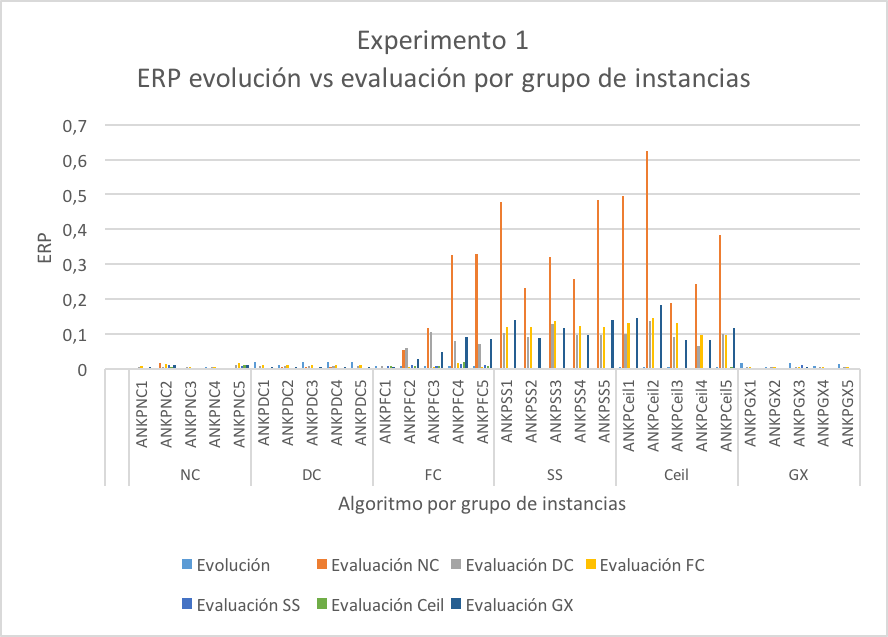
\includegraphics[width=13cm]{images/cap6/evol_vs_eval_exp1.png}
    \captionof{figure}{ERP de cada algoritmo por grupo sobre el conjunto de evaluación y evolución para el experimento 1 (Elaboración propia, 2015) }\label{fig:evol_vs_eval_exp1}
\endgroup

\begingroup
    \centering
    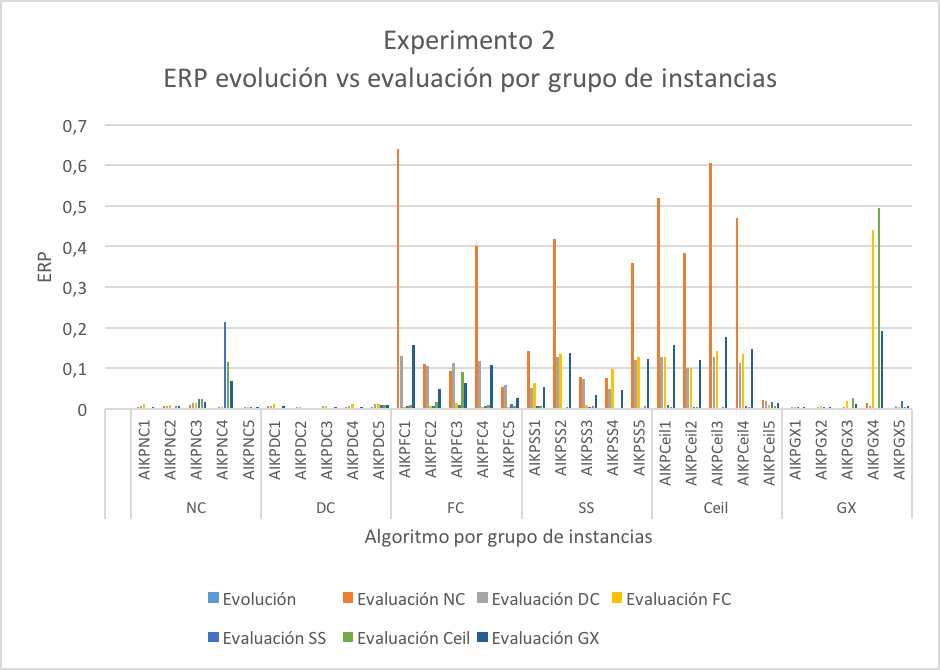
\includegraphics[width=13cm]{images/cap6/evol_vs_eval_exp2.png}
    \captionof{figure}{ERP de cada algoritmo por grupo sobre el conjunto de evaluación y evolución para el experimento 2 (Elaboración propia, 2015)}\label{fig:evol_vs_eval_exp2}
\endgroup

Los resultados obtenidos por los algoritmos producidos se sobre-especializan en el tipo de instancias de entrenamiento (evolución). Esta observación se desprende de la clasificación realizada para las instancias de acuerdo a su tipo. Como se muestra en la Tabla \ref{tab:evol_vs_eval_completa_exp1} para el experimento 1 y la Tabla \ref{tab:evol_vs_eval_completa_exp2} para el experimento 2, los resultados son similares para las instancias que tienen el mismo grupo de evolución y evaluación. Mientras que, para los otros casos, en su mayoría los resultados difieren.


\begin{table}[hbtp!]
\caption{Resultados del ERP para las instancias de evolución y evaluación para el mejor algoritmo de cada sub-experimento del experimento 1}\label{tab:evol_vs_eval_completa_exp1}
\small
\centering
\begin{center}
\rowcolors{2}{gray!25}{white}
\begin{tabular}{cc|cccccc}
\multicolumn{2}{c|}{{\textbf{}}} & \multicolumn{6}{c}{{\textbf{Grupos de instancias de evaluación}}} \\ \hline
{\textbf{Nombre}} & {\textbf{Evolución}} & {\textbf{NC}} & {\textbf{DC}} & {\textbf{FC}} & {\textbf{SS}} & {\textbf{Ceil}} & {\textbf{GX}} \\ \hline
ANKPNC1 & 0,004 & 0,005 & 0,007 & 0,009 & 0,004 & 0,002 & 0,005 \\
ANKPNC2 & 0,004 & 0,019 & 0,007 & 0,015 & 0,012 & 0,008 & 0,012 \\
ANKPNC3 & 0,004 & 0,004 & 0,007 & 0,008 & 0,003 & 0,002 & 0,005 \\
ANKPNC4 & 0,006 & 0,002 & 0,005 & 0,006 & 0,002 & 0,002 & 0,004 \\
ANKPNC5 & 0,005 & 0,005 & 0,012 & 0,017 & 0,010 & 0,011 & 0,011 \\ \hline
ANKPDC1 & 0,020 & 0,005 & 0,008 & 0,013 & 0,002 & 0,002 & 0,006 \\
ANKPDC2 & 0,012 & 0,007 & 0,010 & 0,013 & 0,003 & 0,003 & 0,007 \\
ANKPDC3 & 0,020 & 0,007 & 0,008 & 0,013 & 0,002 & 0,002 & 0,006 \\
ANKPDC4 & 0,020 & 0,006 & 0,008 & 0,013 & 0,002 & 0,002 & 0,006 \\
ANKPDC5 & 0,020 & 0,005 & 0,008 & 0,013 & 0,003 & 0,002 & 0,006 \\ \hline
ANKPFC1 & 0,010 & 0,003 & 0,008 & 0,005 & 0,008 & 0,008 & 0,006 \\
ANKPFC2 & 0,010 & 0,054 & 0,061 & 0,006 & 0,013 & 0,008 & 0,029 \\
ANKPFC3 & 0,009 & 0,118 & 0,106 & 0,007 & 0,009 & 0,010 & 0,050 \\
ANKPFC4 & 0,008 & 0,328 & 0,081 & 0,018 & 0,015 & 0,022 & 0,093 \\
ANKPFC5 & 0,010 & 0,330 & 0,073 & 0,006 & 0,013 & 0,008 & 0,086 \\ \hline
ANKPSS1 & 0,002 & 0,479 & 0,103 & 0,121 & 0,002 & 0,005 & 0,142 \\
ANKPSS2 & 0,002 & 0,233 & 0,092 & 0,121 & 0,002 & 0,005 & 0,091 \\
ANKPSS3 & 0,002 & 0,321 & 0,128 & 0,137 & 0,002 & 0,005 & 0,118 \\
ANKPSS4 & 0,002 & 0,257 & 0,097 & 0,125 & 0,002 & 0,005 & 0,097 \\
ANKPSS5 & 0,002 & 0,484 & 0,099 & 0,120 & 0,003 & 0,004 & 0,142 \\ \hline
ANKPCeil1 & 0,005 & 0,495 & 0,100 & 0,132 & 0,003 & 0,005 & 0,147 \\
ANKPCeil2 & 0,006 & 0,623 & 0,139 & 0,145 & 0,003 & 0,005 & 0,183 \\
ANKPCeil3 & 0,005 & 0,190 & 0,093 & 0,131 & 0,004 & 0,004 & 0,084 \\
ANKPCeil4 & 0,005 & 0,243 & 0,065 & 0,098 & 0,004 & 0,004 & 0,083 \\
ANKPCeil5 & 0,007 & 0,385 & 0,101 & 0,099 & 0,004 & 0,005 & 0,119 \\ \hline
ANKPGX1 & 0,018 & 0,002 & 0,006 & 0,006 & 0,004 & 0,002 & 0,004 \\
ANKPGX2 & 0,008 & 0,002 & 0,006 & 0,006 & 0,002 & 0,002 & 0,004 \\
ANKPGX3 & 0,017 & 0,002 & 0,006 & 0,006 & 0,011 & 0,003 & 0,006 \\
ANKPGX4 & 0,008 & 0,002 & 0,006 & 0,006 & 0,004 & 0,002 & 0,004 \\
ANKPGX5 & 0,015 & 0,002 & 0,006 & 0,006 & 0,002 & 0,003 & 0,004 \\
\hline
\end{tabular}
\end{center}
\caption*{(Elaboración propia, 2015)}
\end{table}

\begin{table}[hbtp!]
\caption{Resultados del ERP para las instancias de evolución y evaluación para el mejor algoritmo de cada sub-experimento del experimento 2}\label{tab:evol_vs_eval_completa_exp2}
\small
\centering
\begin{center}
\rowcolors{2}{gray!25}{white}
\begin{tabular}{cc|cccccc}
\multicolumn{2}{c|}{{\textbf{}}} & \multicolumn{6}{c}{{\textbf{Grupos de instancias de evaluación}}} \\ \hline
{\textbf{Nombre}} & {\textbf{Evolución}} & {\textbf{NC}} & {\textbf{DC}} & {\textbf{FC}} & {\textbf{SS}} & {\textbf{Ceil}} & {\textbf{GX}} \\ \hline
AIKPNC1 & 0,0050 & 0,0048 & 0,0083 & 0,0131 & 0,0030 & 0,0021 & 0,0063 \\
AIKPNC2 & 0,0050 & 0,0067 & 0,0087 & 0,0102 & 0,0024 & 0,0070 & 0,0070 \\
AIKPNC3 & 0,0059 & 0,0112 & 0,0161 & 0,0154 & 0,0237 & 0,0242 & 0,0181 \\
AIKPNC4 & 0,0060 & 0,0035 & 0,0057 & 0,0060 & 0,2135 & 0,1156 & 0,0689 \\
AIKPNC5 & 0,0060 & 0,0022 & 0,0058 & 0,0061 & 0,0042 & 0,0024 & 0,0041 \\ \hline
AIKPDC1 & 0,0197 & 0,0068 & 0,0082 & 0,0131 & 0,0024 & 0,0020 & 0,0065 \\
AIKPDC2 & 0,0182 & 0,0023 & 0,0056 & 0,0060 & 0,0024 & 0,0025 & 0,0038 \\
AIKPDC3 & 0,0172 & 0,0029 & 0,0065 & 0,0070 & 0,0025 & 0,0027 & 0,0043 \\
AIKPDC4 & 0,0197 & 0,0048 & 0,0083 & 0,0131 & 0,0030 & 0,0021 & 0,0063 \\
AIKPDC5 & 0,0285 & 0,0063 & 0,0117 & 0,0133 & 0,0105 & 0,0088 & 0,0101 \\ \hline
AIKPFC1 & 0,0101 & 0,6398 & 0,1303 & 0,0060 & 0,0087 & 0,0090 & 0,1588 \\
AIKPFC2 & 0,0101 & 0,1113 & 0,1070 & 0,0081 & 0,0087 & 0,0165 & 0,0503 \\
AIKPFC3 & 0,0089 & 0,0938 & 0,1123 & 0,0146 & 0,0110 & 0,0911 & 0,0646 \\
AIKPFC4 & 0,0101 & 0,4012 & 0,1178 & 0,0060 & 0,0087 & 0,0090 & 0,1085 \\
AIKPFC5 & 0,0101 & 0,0541 & 0,0604 & 0,0061 & 0,0132 & 0,0084 & 0,0285 \\ \hline
AIKPSS1 & 0,0023 & 0,1429 & 0,0527 & 0,0633 & 0,0080 & 0,0081 & 0,0550 \\
AIKPSS2 & 0,0101 & 0,4184 & 0,1287 & 0,1363 & 0,0012 & 0,0046 & 0,1378 \\
AIKPSS3 & 0,0089 & 0,0795 & 0,0741 & 0,0108 & 0,0044 & 0,0064 & 0,0350 \\
AIKPSS4 & 0,0101 & 0,0773 & 0,0503 & 0,0990 & 0,0013 & 0,0036 & 0,0463 \\
AIKPSS5 & 0,0101 & 0,3598 & 0,1196 & 0,1281 & 0,0034 & 0,0063 & 0,1235 \\ \hline
AIKPCeil1 & 0,0060 & 0,5195 & 0,1284 & 0,1270 & 0,0106 & 0,0058 & 0,1583 \\
AIKPCeil2 & 0,0071 & 0,3848 & 0,1022 & 0,1014 & 0,0041 & 0,0054 & 0,1196 \\
AIKPCeil3 & 0,0061 & 0,6045 & 0,1273 & 0,1434 & 0,0033 & 0,0041 & 0,1765 \\
AIKPCeil4 & 0,0060 & 0,4693 & 0,1144 & 0,1363 & 0,0086 & 0,0048 & 0,1467 \\
AIKPCeil5 & 0,0079 & 0,0221 & 0,0209 & 0,0107 & 0,0175 & 0,0074 & 0,0157 \\ \hline
AIKPGX1 & 0,0165 & 0,0023 & 0,0058 & 0,0060 & 0,0041 & 0,0024 & 0,0041 \\
AIKPGX2 & 0,0066 & 0,0035 & 0,0059 & 0,0079 & 0,0040 & 0,0023 & 0,0047 \\
AIKPGX3 & 0,0158 & 0,0022 & 0,0059 & 0,0188 & 0,0024 & 0,0281 & 0,0115 \\
AIKPGX4 & 0,0081 & 0,0157 & 0,0078 & 0,4410 & 0,0024 & 0,4945 & 0,1923 \\
AIKPGX5 & 0,0155 & 0,0027 & 0,0063 & 0,0061 & 0,0188 & 0,0049 & 0,0078 \\
\hline
\end{tabular}
\end{center}
\caption*{(Elaboración propia, 2015)}
\end{table}

Los algoritmos obtenidos mediante la evolución utilizando el grupo de instancias de adaptación $SS$ y $Ceil$, muestran una clara sobre especialización en las instancias que corresponden al mismo grupo. Estos grupos, como se mencionó en el diseño del experimento, poseen características muy similares. Específicamente, cuando se utilizaron para evolucionar los algoritmos, las instancias del grupo $SS$, surgieron los algoritmos $ANKPSS1$ a $ANKPSS5$ para el experimento 1 y los algoritmos $AIKPSS1$ a $AIKPSS5$ para el experimento 2. En la Tabla \ref{tab:evol_vs_eval_ss} se observan los resultados obtenidos para los cinco algoritmos de cada experimento con las instancias de evolución, solo para los algoritmos del grupo $SS$. Al observar los cinco algoritmos se detectan diferencias estructurales y también diferencias en el desempeño computacional. El mejor algoritmo obtenido es $ANKPSS4$ que presenta un error relativo promedio de $0,22\%$ en las 12 instancias de evolución. La estructura sintáctica del algoritmo se presenta en la Figura \ref{fig:ANKPSS4}. En esta figura se ve que el algoritmo utiliza como elementos la incorporación de nuevos ítems a la mochila por el menor beneficio, mayor peso, mayor ganancia ($beneficio / peso$), los que solo se preocupan de llenar la mochila. Entonces, el algoritmo opera estos terminales alternadamente hasta completar la mochila. Además, los terminales que agregan ítems de acuerdo al peso parecen ser los responsables finales de la especialización para este tipo de instancias. Es decir, el algoritmo $ANKPSS4$ se ha sobre especializado para las instancias de entrenamiento. Esta sobre especialización afecta en mayor medida a este grupo y al grupo $Ceil$, ya que, al tener una relación de igualdad (para el caso $SS$) y casi de igualdad (caso $Ceil$) entre el peso y el beneficio de los ítems a ingresar a la mochila, los algoritmos solo intentan llenar la mochila hasta alcanzar su capacidad. Como resultado, estos algoritmos en particular, obtienen los peores resultados al ser evaluados con los grupos de instancias distintas al de evolución.

\begin{table}[hbtp!]
\caption{Resultados del ERP de los algoritmos obtenidos por el grupo de instancias $SS$ para cada uno de los grupos de instancias de evaluación}\label{tab:evol_vs_eval_ss}
\small
\centering
\begin{center}
\begin{tabular}{ccc|cccccc}
\multicolumn{3}{c|}{{\textbf{}}} & \multicolumn{6}{c}{{\textbf{Grupos de instancias de evaluación}}} \\ \hline
{\textbf{Experimento}} & {\textbf{Nombre}} & {\textbf{Evolución}} & {\textbf{NC}} & {\textbf{DC}} & {\textbf{FC}} & {\textbf{SS}} & {\textbf{Ceil}} & {\textbf{GX}} \\ \hline
\begin{tabular}[c]{@{}c@{}} 
	Experimento 1 \\ SS 
\end{tabular} 		& 	\begin{tabular}[c]{@{}c@{}} ANKPSS1 \\ ANKPSS2 \\ ANKPSS3 \\ ANKPSS4 \\ ANKPSS5 \end{tabular} &
                        \begin{tabular}[c]{@{}c@{}} 0,002 \\ 0,002 \\ 0,002 \\ 0,002 \\ 0,002 \end{tabular} &
                        \begin{tabular}[c]{@{}c@{}} 0,479 \\ 0,233 \\ 0,321 \\ 0,257 \\ 0,484  \end{tabular} &
                        \begin{tabular}[c]{@{}c@{}} 0,103 \\ 0,092 \\ 0,128 \\ 0,097 \\ 0,099  \end{tabular} &
                        \begin{tabular}[c]{@{}c@{}} 0,121 \\ 0,121 \\ 0,137 \\ 0,125 \\ 0,120  \end{tabular} &
                        \begin{tabular}[c]{@{}c@{}} 0,002 \\ 0,002 \\ 0,002 \\ 0,002 \\ 0,003  \end{tabular} &
                        \begin{tabular}[c]{@{}c@{}} 0,005 \\ 0,005 \\ 0,005 \\ 0,005 \\ 0,004  \end{tabular} &
                        \begin{tabular}[c]{@{}c@{}} 0,142 \\ 0,091 \\ 0,118 \\ 0,097 \\ 0,142  \end{tabular} \\ \hline

\begin{tabular}[c]{@{}c@{}} 
	Experimento 2 \\ SS 
\end{tabular} 		& 	\begin{tabular}[c]{@{}c@{}} AIKPSS1 \\ AIKPSS2 \\ AIKPSS3 \\ AIKPSS4 \\ AIKPSS5 \end{tabular} &
                        \begin{tabular}[c]{@{}c@{}} 0,0023 \\ 0,0101 \\ 0,0089 \\ 0,0101 \\ 0,0101 \end{tabular} &
                        \begin{tabular}[c]{@{}c@{}} 0,1429 \\ 0,4184 \\ 0,0795 \\ 0,0773 \\ 0,3598 \end{tabular} &
                        \begin{tabular}[c]{@{}c@{}} 0,0527 \\ 0,1287 \\ 0,0741 \\ 0,0503 \\ 0,1196 \end{tabular} &
                        \begin{tabular}[c]{@{}c@{}} 0,0633 \\ 0,1363 \\ 0,0108 \\ 0,0990 \\ 0,1281 \end{tabular} &
                        \begin{tabular}[c]{@{}c@{}} 0,0080 \\ 0,0012 \\ 0,0044 \\ 0,0013 \\ 0,0034 \end{tabular} &
                        \begin{tabular}[c]{@{}c@{}} 0,0081 \\ 0,0046 \\ 0,0064 \\ 0,0036 \\ 0,0063 \end{tabular} &
                        \begin{tabular}[c]{@{}c@{}} 0,0550 \\ 0,1378 \\ 0,0350 \\ 0,0463 \\ 0,1235 \end{tabular} \\
\hline
\end{tabular}
\end{center}
\caption*{(Elaboración propia, 2015)}
\end{table}

\begingroup
    \centering
    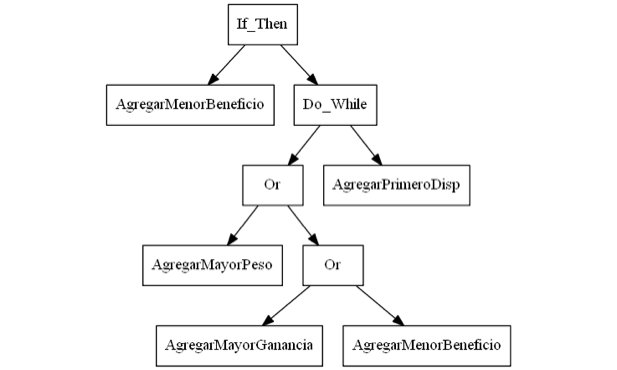
\includegraphics[width=13cm]{images/cap6/ANKPSS4.png}
    \captionof{figure}{Mejor algoritmo del experimento 1 para el grupo de instancias $SS$ (Elaboración propia, 2015)}\label{fig:ANKPSS4}
\endgroup

La sobre-especialización de los algoritmos se puede constatar simplemente revisando los resultados de su evaluación con instancias distintas del mismo grupo. Como se mencionó anteriormente, las tablas \ref{tab:evol_vs_eval_completa_exp1} y \ref{tab:evol_vs_eval_completa_exp2} presentan los resultados del ERP de los cinco algoritmos de cada sub-experimento para distintos grupos de instancias de cada experimento. Se observa que, en general, los algoritmos tienen un mejor rendimiento con las instancias del mismo grupo con el que se utilizaron las instancias para los casos de adaptación (evolución) en comparación a su rendimiento con las instancias de otros grupos. Las instancias del grupo $NC$, $DC$, $FC$, $Ceil$ y $GX$ siguen la misma lógica. Los resultados de la sobre especialización también son constatados para los otros grupos. Una clara excepción a esta sobre-especialización, es lo que ocurre en los grupos $NC$, $DC$, $FC$ y $GX$ al ser evaluados sobre los grupos $SS$ y $Ceil$. Esto se debe a que estas instancias “simplifican” el problema de estudio. Esta simplificación puede ser interpretada como “solo se debe llenar la mochila” y no a “llenar la mochila maximizando la ganancia” y se debe a que estas instancias poseen igualdad o una similitud entre el peso y beneficio que provee cada ítem al ser agregado a la mochila. La particularidad de estos grupos presenta menor dificultad para las funciones y terminales propuestos, generando que los algoritmos que han sido entrenados con otros grupos de instancias con características distintas, posean una mayor facilidad al momento de resolver las instancias de los grupos $SS$ y $Ceil$.

Los algoritmos obtenidos mediante la evolución utilizando el grupo de instancias combinadas $GX$, obtiene resultados similares a los obtenidos por otros algoritmos que evolucionaron con un solo grupo de adaptación. En la Tabla \ref{tab:evol_vs_eval_gx} se muestran los resultados que obtienen los algoritmos $ANKPGX1$ a $ANKPGX5$ para el proceso de evaluación con los distintos grupos del experimento 1. Es posible apreciar que los resultados obtenidos mediante la evolución utilizando instancias de diversos grupos, no posee una sobre especialización como ocurre con los otros algoritmos. Esto es debido a que los algoritmos se adaptan a una mayor cantidad de instancias, las que presentan una variación en la dificultad y características específicas que posee cada una para ser resuelta. En la Tabla \ref{tab:evol_vs_eval_gx} también se muestran los resultados que obtienen los algoritmos $AIKPGX1$ a $AIKPGX5$ para el proceso de evaluación con los distintos grupos del experimento 2, donde se puede constatar que ocurre un efecto similar al producido en el experimento 1.

\begin{table}[hbtp!]
\caption{Resultados del ERP de los algoritmos obtenidos por el grupo de instancias $GX$ para cada uno de los grupos de instancias de evaluación}\label{tab:evol_vs_eval_gx}
\small
\centering
\begin{center}
\begin{tabular}{ccc|cccccc}
\multicolumn{3}{c|}{{\textbf{}}} & \multicolumn{6}{c}{{\textbf{Grupos de instancias de evaluación}}} \\ \hline
{\textbf{Experimento}} & {\textbf{Nombre}} & {\textbf{Evolución}} & {\textbf{NC}} & {\textbf{DC}} & {\textbf{FC}} & {\textbf{SS}} & {\textbf{Ceil}} & {\textbf{GX}} \\ \hline
\begin{tabular}[c]{@{}c@{}} 
	Exp. 1 \\ GX 
\end{tabular} 		& 	\begin{tabular}[c]{@{}c@{}} ANKPGX1 \\ ANKPGX2 \\ ANKPGX3 \\ ANKPGX4 \\ ANKPGX5 \end{tabular} &
                        \begin{tabular}[c]{@{}c@{}} 0,0176 \\ 0,0077 \\ 0,0172 \\ 0,0081 \\ 0,0149 \end{tabular} &
                        \begin{tabular}[c]{@{}c@{}} 0,0022 \\ 0,0022 \\ 0,0022 \\ 0,0022 \\ 0,0022 \end{tabular} &
                        \begin{tabular}[c]{@{}c@{}} 0,0057 \\ 0,0059 \\ 0,0057 \\ 0,0057 \\ 0,0059 \end{tabular} &
                        \begin{tabular}[c]{@{}c@{}} 0,0060 \\ 0,0060 \\ 0,0060 \\ 0,0060 \\ 0,0061 \end{tabular} &
                        \begin{tabular}[c]{@{}c@{}} 0,0041 \\ 0,0024 \\ 0,0111 \\ 0,0041 \\ 0,0024 \end{tabular} &
                        \begin{tabular}[c]{@{}c@{}} 0,0024 \\ 0,0025 \\ 0,0029 \\ 0,0024 \\ 0,0026 \end{tabular} &
                        \begin{tabular}[c]{@{}c@{}} 0,0041 \\ 0,0038 \\ 0,0056 \\ 0,0041 \\ 0,0038 \end{tabular} \\ \hline

\begin{tabular}[c]{@{}c@{}} 
    Exp. 2 \\ GX 
\end{tabular}       &   \begin{tabular}[c]{@{}c@{}} AIKPGX1 \\ AIKPGX2 \\ AIKPGX3 \\ AIKPGX4 \\ AIKPGX5 \end{tabular} &
                        \begin{tabular}[c]{@{}c@{}} 0,0165 \\ 0,0066 \\ 0,0158 \\ 0,0081 \\ 0,0155 \end{tabular} &
                        \begin{tabular}[c]{@{}c@{}} 0,0023 \\ 0,0035 \\ 0,0022 \\ 0,0157 \\ 0,0027 \end{tabular} &
                        \begin{tabular}[c]{@{}c@{}} 0,0058 \\ 0,0059 \\ 0,0059 \\ 0,0078 \\ 0,0063 \end{tabular} &
                        \begin{tabular}[c]{@{}c@{}} 0,0060 \\ 0,0079 \\ 0,0188 \\ 0,4410 \\ 0,0061 \end{tabular} &
                        \begin{tabular}[c]{@{}c@{}} 0,0041 \\ 0,0040 \\ 0,0024 \\ 0,0024 \\ 0,0188 \end{tabular} &
                        \begin{tabular}[c]{@{}c@{}} 0,0024 \\ 0,0023 \\ 0,0281 \\ 0,4945 \\ 0,0049 \end{tabular} &
                        \begin{tabular}[c]{@{}c@{}} 0,0041 \\ 0,0047 \\ 0,0115 \\ 0,1923 \\ 0,0078 \end{tabular} \\
\hline
\end{tabular}
\end{center}
\caption*{(Elaboración propia, 2015)}
\end{table}

Los algoritmos producidos son muy rápidos para resolver los problemas de la mochila. En la Tabla \ref{tab:evol_vs_eval_tiempos_exp1} se muestra el tiempo que le toma al mejor algoritmo de cada ejecución resolver las instancias de cada uno de los grupos ($NC$, $DC$, $FC$, $SS$ y $Ceil$) para el experimento 1. Es importante destacar que cada uno de los grupos contiene 780 instancias que varían en tamaño de $100$ a $10.000$ ítems y el grupo GX contiene las $3.900$ instancias de los otros grupos (véase \ref{cap:sel_casos_adapt_pm01}). El tiempo empleado es en promedio cinco minutos, alcanzando menos de dos minutos el más rápido y casi 12 minutos el más lento de ellos. Adicionalmente, se puede ver que el grupo GX de evaluación (compuesto por todas las instancias de evaluación de los otros grupos) obtiene tiempos promedios de 22 minutos, obteniendo menos de 10 minutos el más rápido y casi una hora el más lento. Los algoritmos más rápidos resuelven en una milésima de segundo cada instancia, mientras que los más lentos las resuelven en aproximadamente un segundo. En la Tabla \ref{tab:evol_vs_eval_tiempos_exp2} se puede observar los tiempos en que los mejores algoritmos del experimento 2 resuelven las instancias para cada uno de los grupos, aunque, si bien los tiempos empleados en la evaluación no son iguales, son similares. Esto se debe a que todos los algoritmos producidos tienen una complejidad polinomial. %Agregar que grupo es más rápido de resolver o cosas así

\begin{table}[hbtp!]
\caption{Tiempo que demora en resolver el mejor algoritmo de cada sub-experimento del experimento 1, los grupos de evaluación}\label{tab:evol_vs_eval_tiempos_exp1}
\small
\centering
\begin{center}
\rowcolors{2}{gray!25}{white}
\begin{tabular}{c|cccccc}
{\textbf{}} & \multicolumn{6}{c}{{\textbf{Tiempo en minutos}}} \\ \hline
{\textbf{Nombre}} & {\textbf{NC}} & {\textbf{DC}} & {\textbf{FC}} & {\textbf{SS}} & {\textbf{Ceil}} & {\textbf{GX}} \\ \hline
ANKPNC1 & 5,36 & 4,26 & 5,83 & 3,41 & 4,77 & 23,62 \\
ANKPNC2 & 7,39 & 5,34 & 7,55 & 3,75 & 5,93 & 29,97 \\
ANKPNC3 & 5,32 & 4,12 & 5,73 & 3,33 & 4,58 & 23,08 \\
ANKPNC4 & 4,35 & 3,47 & 4,68 & 2,81 & 3,95 & 19,26 \\
ANKPNC5 & 4,72 & 3,59 & 4,92 & 2,82 & 3,86 & 19,91 \\
ANKPDC1 & 5,80 & 4,40 & 6,49 & 3,36 & 5,09 & 25,14 \\
ANKPDC2 & 6,67 & 5,33 & 6,56 & 3,44 & 5,73 & 27,72 \\
ANKPDC3 & 6,89 & 5,36 & 7,81 & 4,17 & 6,01 & 30,24 \\
ANKPDC4 & 4,67 & 3,65 & 5,26 & 2,89 & 4,18 & 20,65 \\
ANKPDC5 & 4,66 & 3,61 & 5,07 & 2,80 & 3,87 & 20,02 \\
ANKPFC1 & 5,78 & 4,44 & 6,36 & 3,39 & 5,20 & 25,17 \\
ANKPFC2 & 5,13 & 5,05 & 5,33 & 4,56 & 5,54 & 25,61 \\
ANKPFC3 & 11,82 & 11,68 & 11,46 & 11,37 & 11,25 & 57,58 \\
ANKPFC4 & 4,09 & 4,43 & 4,59 & 3,79 & 4,23 & 21,13 \\
ANKPFC5 & 4,54 & 4,72 & 4,84 & 3,80 & 4,50 & 22,39 \\
ANKPSS1 & 1,93 & 1,87 & 1,89 & 1,90 & 1,88 & 9,49 \\
ANKPSS2 & 2,49 & 1,78 & 1,80 & 1,86 & 1,91 & 9,83 \\
ANKPSS3 & 6,60 & 5,86 & 4,34 & 4,91 & 4,99 & 26,71 \\
ANKPSS4 & 2,32 & 1,72 & 1,80 & 1,81 & 1,80 & 9,44 \\
ANKPSS5 & 1,82 & 1,82 & 1,87 & 1,87 & 1,81 & 9,19 \\
ANKPCeil1 & 2,94 & 3,22 & 2,64 & 2,32 & 2,83 & 13,96 \\
ANKPCeil2 & 2,63 & 3,16 & 2,33 & 2,55 & 2,64 & 13,31 \\
ANKPCeil3 & 7,91 & 4,97 & 5,04 & 4,08 & 4,96 & 26,97 \\
ANKPCeil4 & 3,80 & 3,61 & 3,22 & 2,46 & 3,36 & 16,44 \\
ANKPCeil5 & 4,31 & 4,59 & 3,56 & 2,82 & 3,95 & 19,24 \\
ANKPGX1 & 4,59 & 3,70 & 5,14 & 2,92 & 4,20 & 20,55 \\
ANKPGX2 & 4,55 & 3,64 & 5,29 & 2,88 & 4,44 & 20,80 \\
ANKPGX3 & 9,02 & 7,04 & 10,03 & 4,84 & 7,72 & 38,64 \\
ANKPGX4 & 4,55 & 3,62 & 5,14 & 2,91 & 4,20 & 20,41 \\
ANKPGX5 & 5,58 & 4,35 & 6,14 & 3,33 & 4,68 & 24,09 \\
\hline
\end{tabular}
\end{center}
\caption*{(Elaboración propia, 2015)}
\end{table}

\begin{table}[hbtp!]
\caption{Tiempo que demora en resolver el mejor algoritmo de cada sub-experimento del experimento 2, los grupos de evaluación}\label{tab:evol_vs_eval_tiempos_exp2}
\small
\centering
\begin{center}
\rowcolors{2}{gray!25}{white}
\begin{tabular}{c|cccccc}
{\textbf{}} & \multicolumn{6}{c}{{\textbf{Tiempo en minutos}}} \\ \hline
{\textbf{Nombre}} & {\textbf{NC}} & {\textbf{DC}} & {\textbf{FC}} & {\textbf{SS}} & {\textbf{Ceil}} & {\textbf{GX}} \\ \hline
AIKPNC1 & 4,68 & 3,67 & 5,34 & 3,00 & 4,84 & 21,53 \\
AIKPNC2 & 10,31 & 8,04 & 11,18 & 6,16 & 10,97 & 46,66 \\
AIKPNC3 & 6,87 & 5,30 & 7,73 & 4,15 & 5,90 & 29,95 \\
AIKPNC4 & 10,20 & 7,95 & 11,22 & 2,10 & 4,82 & 36,28 \\
AIKPNC5 & 4,58 & 3,59 & 4,90 & 2,81 & 3,92 & 19,80 \\
AIKPDC1 & 6,87 & 5,43 & 7,72 & 4,35 & 6,22 & 30,60 \\
AIKPDC2 & 5,83 & 4,39 & 6,33 & 3,51 & 5,17 & 25,23 \\
AIKPDC3 & 5,68 & 4,41 & 6,38 & 3,55 & 5,16 & 25,17 \\
AIKPDC4 & 4,62 & 3,66 & 5,17 & 2,99 & 4,24 & 20,68 \\
AIKPDC5 & 4,60 & 3,51 & 4,99 & 2,82 & 3,84 & 19,77 \\
AIKPFC1 & 4,29 & 6,10 & 6,14 & 6,16 & 6,13 & 28,82 \\
AIKPFC2 & 6,42 & 7,00 & 6,38 & 6,40 & 6,20 & 32,41 \\
AIKPFC3 & 17,12 & 9,37 & 5,32 & 5,20 & 3,85 & 40,87 \\
AIKPFC4 & 4,52 & 5,07 & 5,10 & 5,06 & 4,97 & 24,71 \\
AIKPFC5 & 5,12 & 4,88 & 5,04 & 4,05 & 4,53 & 23,61 \\
AIKPSS1 & 9,61 & 32,65 & 2,95 & 2,95 & 4,09 & 52,24 \\
AIKPSS2 & 3,02 & 3,00 & 2,46 & 2,56 & 2,80 & 13,84 \\
AIKPSS3 & 5,65 & 4,89 & 6,12 & 4,66 & 5,15 & 26,47 \\
AIKPSS4 & 4,05 & 2,93 & 3,51 & 2,49 & 3,20 & 16,18 \\
AIKPSS5 & 3,05 & 3,02 & 2,40 & 2,58 & 2,60 & 13,65 \\
AIKPCeil1 & 2,93 & 3,64 & 2,71 & 2,56 & 3,29 & 15,12 \\
AIKPCeil2 & 4,08 & 4,61 & 3,68 & 3,01 & 4,19 & 19,57 \\
AIKPCeil3 & 2,30 & 2,75 & 2,24 & 2,40 & 2,45 & 12,13 \\
AIKPCeil4 & 2,86 & 3,05 & 2,54 & 2,54 & 2,87 & 13,86 \\
AIKPCeil5 & 4,68 & 3,65 & 5,25 & 3,39 & 4,19 & 21,16 \\
AIKPGX1 & 4,73 & 3,72 & 5,25 & 2,87 & 4,31 & 20,88 \\
AIKPGX2 & 5,26 & 4,19 & 5,73 & 3,13 & 4,66 & 22,97 \\
AIKPGX3 & 4,64 & 3,71 & 4,92 & 2,91 & 3,90 & 20,08 \\
AIKPGX4 & 10,03 & 7,79 & 0,34 & 6,05 & 0,44 & 24,64 \\
AIKPGX5 & 5,90 & 4,58 & 6,38 & 3,79 & 4,87 & 25,52 \\
\hline
\end{tabular}
\end{center}
\caption*{(Elaboración propia, 2015)}
\end{table}

Los algoritmos obtenidos mediante el proceso co-evolutivo utilizando el método de islas tienen un desempeño computacional similar a los algoritmos obtenidos mediante el proceso tradicional. En las tablas \ref{tab:mejores_exp_hits_pm01} y \ref{tab:mejores_exp_erp_pm01} se muestran los resultados de cinco mejores algoritmos obtenidos para cada experimento. Estos algoritmos fueron los mejores de cada uno de los sub-experimentos de acuerdo a los resultados obtenidos al ser evaluados con los grupos de evaluación. Específicamente, en la Tabla \ref{tab:mejores_exp_hits_pm01} se presentan los mejores individuos de acuerdo a la cantidad de instancias que logran resolver de forma óptima. Mientras que en la Tabla \ref{tab:mejores_exp_erp_pm01} se presentan los mejores individuos que obtuvieron el menor ERP en el grupo de evaluación. En estas tablas se presentan los indicadores de cada algoritmo y el error relativo que se obtuvo al evaluar los algoritmos con el mismo conjunto de instancias de evaluación y la cantidad de soluciones óptimas que encuentra. Tal como se observa, el error relativo promedio de los algoritmos del primer experimento es similar al del segundo experimento. Los resultados obtenidos por ambos experimentos siguen una distribución normal, así lo muestra el \textit{test de Shapiro-Wilk}. En consecuencia,  el \textit{test} de ANOVA que proporciona bajo un 95\% de confiabilidad que no existe diferencia significativa en los datos obtenidos, por lo que no es posible rechazar la hipótesis nula. El resultado contrasta descubrimientos realizados por otros autores para algoritmos genéticos, lo que puede ser inferido puesto que algunos de los resultados obtenidos utilizando el método de la PG con co-evolución muestran una mejora en la calidad de los algoritmos, la que es estadísticamente despreciable.

\begin{table}[hbtp!]
\caption{Mejores individuos por cantidad de soluciones encontradas en grupo de evaluación}\label{tab:mejores_exp_hits_pm01}
\small
\centering
\begin{center}
\begin{tabular}{ccc|ccc|ccc}
\multicolumn{3}{c}{{\textbf{ }}} & \multicolumn{3}{|c|}{{\textbf{Error Relativo}}} & \multicolumn{3}{c}{{\textbf{ }}} \\
{\textbf{Grupo}} & {\textbf{Exp.}} & {\textbf{Nombre}} & {\textbf{Peor}} & {\textbf{Prom.}} & {\textbf{Mejor}} & {\textbf{Soluciones}} & {\textbf{Nodos}} & {\textbf{Altura}}\\ \hline
NC & 	\begin{tabular}[c]{@{}c@{}} 1 \\ 2 \end{tabular} &
		\begin{tabular}[c]{@{}c@{}} ANKPNC4 \\ AIKPNC5 \end{tabular} &
		\begin{tabular}[c]{@{}c@{}} 0,2114 \\ 0,8044   \end{tabular} &
		\begin{tabular}[c]{@{}c@{}} 0,0036 \\ 0,0041   \end{tabular} &
		\begin{tabular}[c]{@{}c@{}} 0 \\ 0 			   \end{tabular} &
		\begin{tabular}[c]{@{}c@{}} 205 \\ 189         \end{tabular} &
		\begin{tabular}[c]{@{}c@{}} 5 \\ 3 			   \end{tabular} &
		\begin{tabular}[c]{@{}c@{}} 15 \\ 5 		   \end{tabular} \\ \hline

DC & 	\begin{tabular}[c]{@{}c@{}} 1 \\ 2 \end{tabular} &
		\begin{tabular}[c]{@{}c@{}} ANKPDC2 \\ AIKPDC1 \end{tabular} &
		\begin{tabular}[c]{@{}c@{}} 1,0000 \\ 0,5933   \end{tabular} &
		\begin{tabular}[c]{@{}c@{}} 0,0073 \\ 0,0065   \end{tabular} &
		\begin{tabular}[c]{@{}c@{}} 0 \\ 0 			   \end{tabular} &
		\begin{tabular}[c]{@{}c@{}} 303 \\ 185         \end{tabular} &
		\begin{tabular}[c]{@{}c@{}} 6 \\ 5 			   \end{tabular} &
		\begin{tabular}[c]{@{}c@{}} 15 \\ 13 		   \end{tabular} \\ \hline

FC & 	\begin{tabular}[c]{@{}c@{}} 1 \\ 2 \end{tabular} &
		\begin{tabular}[c]{@{}c@{}} ANKPFC1 \\ AIKPFC5 \end{tabular} &
		\begin{tabular}[c]{@{}c@{}} 0,2805 \\ 0,8035   \end{tabular} &
		\begin{tabular}[c]{@{}c@{}} 0,0063 \\ 0,0285   \end{tabular} &
		\begin{tabular}[c]{@{}c@{}} 0 \\ 0 			   \end{tabular} &
		\begin{tabular}[c]{@{}c@{}} 96 \\ 12         \end{tabular} &
		\begin{tabular}[c]{@{}c@{}} 4 \\ 2 			   \end{tabular} &
		\begin{tabular}[c]{@{}c@{}} 14 \\ 3 		   \end{tabular} \\ \hline

SS & 	\begin{tabular}[c]{@{}c@{}} 1 \\ 2 \end{tabular} &
		\begin{tabular}[c]{@{}c@{}} ANKPSS4 \\ AIKPSS4 \end{tabular} &
		\begin{tabular}[c]{@{}c@{}} 0,9027 \\ 0,7692   \end{tabular} &
		\begin{tabular}[c]{@{}c@{}} 0,0972 \\ 0,0463   \end{tabular} &
		\begin{tabular}[c]{@{}c@{}} 0 \\ 0 			   \end{tabular} &
		\begin{tabular}[c]{@{}c@{}} 68 \\ 102          \end{tabular} &
		\begin{tabular}[c]{@{}c@{}} 3 \\ 5 			   \end{tabular} &
		\begin{tabular}[c]{@{}c@{}} 5 \\ 11 		   \end{tabular} \\ \hline

Ceil & 	\begin{tabular}[c]{@{}c@{}} 1 \\ 2 \end{tabular} &
		\begin{tabular}[c]{@{}c@{}} ANKPCeil2 \\ AIKPCeil3 \end{tabular} &
		\begin{tabular}[c]{@{}c@{}} 0,9790 \\ 0,9790   \end{tabular} &
		\begin{tabular}[c]{@{}c@{}} 0,1830 \\ 0,1765   \end{tabular} &
		\begin{tabular}[c]{@{}c@{}} 0 \\ 0 			   \end{tabular} &
		\begin{tabular}[c]{@{}c@{}} 67 \\ 65          \end{tabular} &
		\begin{tabular}[c]{@{}c@{}} 5 \\ 6 			   \end{tabular} &
		\begin{tabular}[c]{@{}c@{}} 13 \\ 15 		   \end{tabular} \\ \hline

GX & 	\begin{tabular}[c]{@{}c@{}} 1 \\ 2 \end{tabular} &
		\begin{tabular}[c]{@{}c@{}} ANKPGX3 \\ AIKPGX2 \end{tabular} &
		\begin{tabular}[c]{@{}c@{}} 0,8363 \\ 0,8044   \end{tabular} &
		\begin{tabular}[c]{@{}c@{}} 0,0056 \\ 0,0047   \end{tabular} &
		\begin{tabular}[c]{@{}c@{}} 0 \\ 0 			   \end{tabular} &
		\begin{tabular}[c]{@{}c@{}} 215 \\ 192          \end{tabular} &
		\begin{tabular}[c]{@{}c@{}} 4 \\ 5			   \end{tabular} &
		\begin{tabular}[c]{@{}c@{}} 9 \\ 15 		   \end{tabular} \\
\hline
\end{tabular}
\end{center}
\caption*{(Elaboración propia, 2015)}
\end{table}

\begin{table}[hbtp!]
\caption{Mejores individuos por menor ERP en grupo de evaluación}\label{tab:mejores_exp_erp_pm01}
\small
\centering
\begin{center}
\begin{tabular}{ccc|ccc|ccc}
\multicolumn{3}{c}{{\textbf{ }}} & \multicolumn{3}{|c|}{{\textbf{Error Relativo}}} & \multicolumn{3}{c}{{\textbf{ }}} \\
{\textbf{Grupo}} & {\textbf{Exp.}} & {\textbf{Nombre}} & {\textbf{Peor}} & {\textbf{Prom.}} & {\textbf{Mejor}} & {\textbf{Soluciones}} & {\textbf{Nodos}} & {\textbf{Altura}}\\ \hline
NC & 	\begin{tabular}[c]{@{}c@{}} 1 \\ 2 \end{tabular} &
		\begin{tabular}[c]{@{}c@{}} ANKPNC4 \\ AIKPNC5 \end{tabular} &
		\begin{tabular}[c]{@{}c@{}} 0,2114 \\ 0,8044   \end{tabular} &
		\begin{tabular}[c]{@{}c@{}} 0,0036 \\ 0,0041   \end{tabular} &
		\begin{tabular}[c]{@{}c@{}} 0 \\ 0 			   \end{tabular} &
		\begin{tabular}[c]{@{}c@{}} 205 \\ 189         \end{tabular} &
		\begin{tabular}[c]{@{}c@{}} 5 \\ 3 			   \end{tabular} &
		\begin{tabular}[c]{@{}c@{}} 15 \\ 5 		   \end{tabular} \\ \hline

DC & 	\begin{tabular}[c]{@{}c@{}} 1 \\ 2 \end{tabular} &
		\begin{tabular}[c]{@{}c@{}} ANKPDC1 \\ AIKPDC2 \end{tabular} &
		\begin{tabular}[c]{@{}c@{}} 0,5933 \\  0,2114  \end{tabular} &
		\begin{tabular}[c]{@{}c@{}} 0,0060 \\  0,0038  \end{tabular} &
		\begin{tabular}[c]{@{}c@{}} 0 \\ 0 			   \end{tabular} &
		\begin{tabular}[c]{@{}c@{}} 188 \\ 178         \end{tabular} &
		\begin{tabular}[c]{@{}c@{}} 6 \\ 6 			   \end{tabular} &
		\begin{tabular}[c]{@{}c@{}} 14 \\ 15 		   \end{tabular} \\ \hline

FC & 	\begin{tabular}[c]{@{}c@{}} 1 \\ 2 \end{tabular} &
		\begin{tabular}[c]{@{}c@{}} ANKPFC1 \\ AIKPFC5 \end{tabular} &
		\begin{tabular}[c]{@{}c@{}} 0,2805 \\ 0,8035   \end{tabular} &
		\begin{tabular}[c]{@{}c@{}} 0,0063 \\ 0,0285   \end{tabular} &
		\begin{tabular}[c]{@{}c@{}} 0 \\ 0 			   \end{tabular} &
		\begin{tabular}[c]{@{}c@{}} 96 \\ 12         \end{tabular} &
		\begin{tabular}[c]{@{}c@{}} 4 \\ 2 			   \end{tabular} &
		\begin{tabular}[c]{@{}c@{}} 14 \\ 3 		   \end{tabular} \\ \hline

SS & 	\begin{tabular}[c]{@{}c@{}} 1 \\ 2 \end{tabular} &
		\begin{tabular}[c]{@{}c@{}} ANKPSS2 \\ AIKPSS3 \end{tabular} &
		\begin{tabular}[c]{@{}c@{}} 0,8590 \\ 0,7056   \end{tabular} &
		\begin{tabular}[c]{@{}c@{}} 0,0905 \\ 0,0350   \end{tabular} &
		\begin{tabular}[c]{@{}c@{}} 0 \\ 0 			   \end{tabular} &
		\begin{tabular}[c]{@{}c@{}} 63 \\ 10           \end{tabular} &
		\begin{tabular}[c]{@{}c@{}} 4 \\ 4 			   \end{tabular} &
		\begin{tabular}[c]{@{}c@{}} 10 \\ 13		   \end{tabular} \\ \hline

Ceil & 	\begin{tabular}[c]{@{}c@{}} 1 \\ 2 \end{tabular} &
		\begin{tabular}[c]{@{}c@{}} ANKPCeil4 \\ AIKPCeil5 \end{tabular} &
		\begin{tabular}[c]{@{}c@{}} 0,9299 \\ 0,9391   \end{tabular} &
		\begin{tabular}[c]{@{}c@{}} 0,0830 \\ 0,0157   \end{tabular} &
		\begin{tabular}[c]{@{}c@{}} 0 \\ 0 			   \end{tabular} &
		\begin{tabular}[c]{@{}c@{}} 48 \\ 53           \end{tabular} &
		\begin{tabular}[c]{@{}c@{}} 4 \\ 6 			   \end{tabular} &
		\begin{tabular}[c]{@{}c@{}} 11 \\ 14 		   \end{tabular} \\ \hline

GX & 	\begin{tabular}[c]{@{}c@{}} 1 \\ 2 \end{tabular} &
		\begin{tabular}[c]{@{}c@{}} ANKPGX2 \\ AIKPGX1 \end{tabular} &
		\begin{tabular}[c]{@{}c@{}} 0,2114 \\ 0,8044   \end{tabular} &
		\begin{tabular}[c]{@{}c@{}} 0,0038 \\ 0,0041   \end{tabular} &
		\begin{tabular}[c]{@{}c@{}} 0 \\ 0 			   \end{tabular} &
		\begin{tabular}[c]{@{}c@{}} 200 \\ 184          \end{tabular} &
		\begin{tabular}[c]{@{}c@{}} 5 \\ 5			   \end{tabular} &
		\begin{tabular}[c]{@{}c@{}} 8 \\ 11 		   \end{tabular} \\
\hline
\end{tabular}
\end{center}
\caption*{(Elaboración propia, 2015)}
\end{table}

\subsection{Estructura de los algoritmos generados}

Para facilitar la comprensión de los algoritmos, en esta sección se presenta una figura que muestra el árbol sintáctico del algoritmo junto a una breve explicación de cómo funciona. Los algoritmos descritos en esta sección incluyen sólo al mejor algoritmo de los que fueron señalados en la Tabla \ref{tab:mejores_exp_hits_pm01} y \ref{tab:mejores_exp_erp_pm01} para cada experimento. Estos algoritmos son $ANKPDC2$ y $AIKPGX2$ para la Tabla \ref{tab:mejores_exp_erp_pm01}, que representan a los mejores algoritmos para el problema de la mochila utilizando como criterio encontrar la mayor cantidad de soluciones óptimas para las instancias de evaluación. Para la Tabla \ref{tab:mejores_exp_hits_pm01} son seleccionados los algoritmos $ANKPNC4$ y $AIKPDC2$ que representan a los mejores algoritmos para el problema de la mochila siguiendo el criterio de obtener el menor ERP para las instancias de evaluación.

\subsubsection{ANKPDC2}

El $ANKPDC2$ es el mejor algoritmo obtenido en el experimento 1, utilizando como criterio la cantidad de soluciones que encuentra en el grupo de evaluación. En la Figura \ref{fig:ANKPDC2} se puede ver el algoritmo por medio de su árbol sintáctico. Este algoritmo posee 15 nodos y una altura de 6, compuesto de 7 terminales y 8 funciones. Este algoritmo sigue una lógica puramente constructiva, utilizando distintos criterios tiene por objetivo el llenado de la mochila.
Los pasos a realizar por este algoritmo inician con el ingreso del elemento con el mayor beneficio. Si se realiza el ingreso, se procede a realizar un ciclo \textit{“while”} con la condición de \textit{“true”}, es decir, se ejecuta el árbol derecho hasta que no se produzcan más cambios. El árbol derecho consta de el ingreso de ítems a la mochila iniciando por el de mayor ganancia, posteriormente el primero de la lista de disponibles y posteriormente se ingresa a otro ciclo que llena todos los elementos restantes de acuerdo a su menor peso. Este proceso se realiza hasta alcanzar la capacidad máxima de la mochila. El terminal “AgregarMayorGanancia” ubicado en la rama derecha no es ejecutado. La lógica de este algoritmo es un goloso con el criterio principal de agregar los ítem que provean la mayor ganancia.

\begingroup
    \centering
    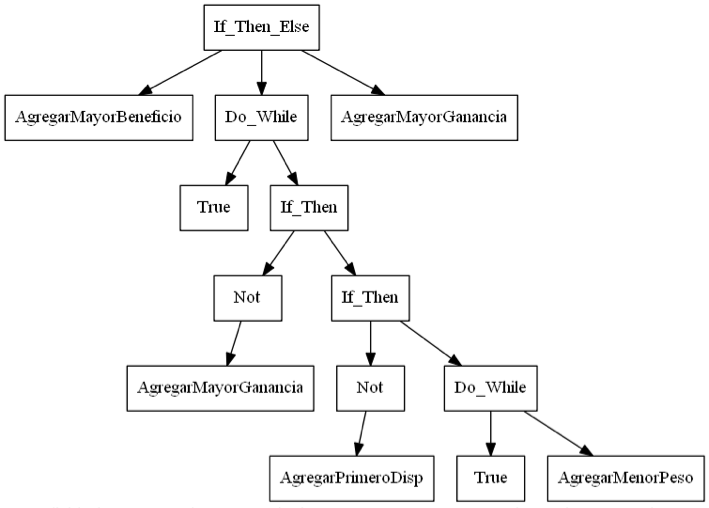
\includegraphics[width=13cm]{images/cap6/ANKPDC2.png}
    \captionof{figure}{Mejor algoritmo del experimento 1 por cantidad de soluciones óptimas obtenidas (Elaboración propia, 2015)}\label{fig:ANKPDC2}
\endgroup

\subsubsection{AIKPGX2}

El $AIKPGX2$ es el mejor algoritmo obtenido en el experimento 2, utilizando como criterio la cantidad de soluciones que encuentra en el grupo de evaluación. En la Figura \ref{fig:AIKPGX2} se puede ver el algoritmo por medio de su árbol sintáctico. Este algoritmo posee 15 nodos y una altura de 5, se encuentra compuesto de 8 terminales y 7 funciones. A diferencia del algoritmo anterior, este algoritmo utiliza un terminal que elimina siguiendo una lógica constructiva y de refinamiento.
Los pasos a realizar por este algoritmo inician con un ciclo \textit{“while”} donde se ingresan ítems de acuerdo a la mayor ganancia y menor peso. Posteriormente, se ejecuta el árbol derecho agregando ítems de acuerdo a su mayor ganancia y mayor beneficio. Si cinco ítems son agregados, se procede a eliminar el ítem con la peor ganancia y se ejecuta nuevamente el algoritmo. La lógica que sigue este algoritmo es de un goloso, que en un determinado momento realiza un refinamiento.

\begingroup
    \centering
    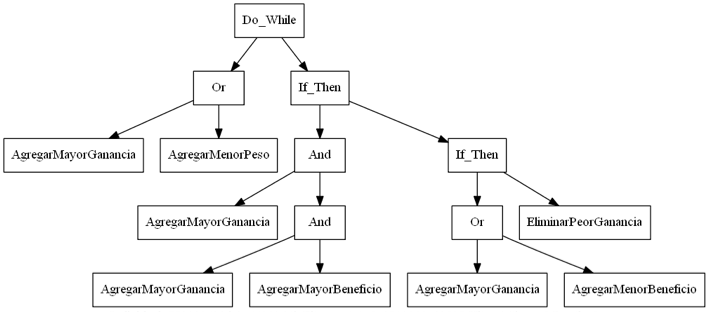
\includegraphics[width=13cm]{images/cap6/AIKPGX2.png}
    \captionof{figure}{Mejor algoritmo del experimento 2 por cantidad de soluciones óptimas obtenidas (Elaboración propia, 2015)}\label{fig:AIKPGX2}
\endgroup

\subsubsection{ANKPNC4}

El $ANKPNC4$ es el mejor algoritmo obtenido en el experimento 1, utilizando como criterio la obtención del menor ERP al ser evaluado en el grupo de evaluación. En la Figura \ref{fig:ANKPNC4} se puede ver el árbol sintáctico del algoritmo. Este algoritmo posee 15 nodos y una altura de 5, está compuesto de 9 terminales y 6 funciones. Este algoritmo sigue una lógica constructiva y de refinamiento.
El algoritmo inicia su procedimiento mediante un ciclo \textit{“while”}. Comienza insertando 3 ítems a la mochila con los criterios de mayor ganancia, primero disponible y menor peso para posteriormente eliminar el con peor beneficio de éstos. A continuación, agrega ítems a la mochila de acuerdo a su mayor ganancia, si no es posible agregar al de mayor ganancia, se procede a agregar el de menor peso. Finalmente, vuelve a comenzar el algoritmo. La lógica de este algoritmo es un goloso con el criterio principal de agregar los ítem que provean la mayor ganancia y en un determinado momento intenta realizar un refinamiento.

\begingroup
    \centering
    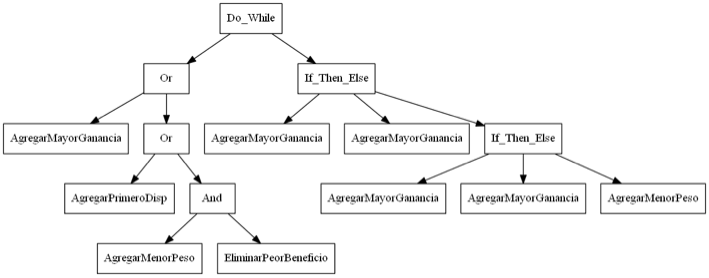
\includegraphics[width=13cm]{images/cap6/ANKPNC4.png}
    \captionof{figure}{Mejor algoritmo del experimento 1 por menor ERP (Elaboración propia, 2015)}\label{fig:ANKPNC4}
\endgroup

\subsubsection{AIKPDC2}

El $AIKPDC2$ es el mejor algoritmo obtenido en el experimento 2, utilizando como criterio la obtención del menor ERP al ser evaluado en el grupo de evaluación. En la Figura \ref{fig:AIKPDC2} se puede ver el árbol sintáctico del algoritmo. Este algoritmo posee 13 nodos y una altura de 5, se compone de 8 terminales y 5 funciones. Este algoritmo sigue una lógica constructiva y de refinamiento.
Este algoritmo inicia con un ciclo \textit{“while”} que se ejecuta hasta llenar la mochila. La construcción se realiza por medio del ingreso de ítems por su mayor beneficio, y posteriormente por su mayor ganancia hasta que la mochila se encuentra llena. A continuación, se entra a un nuevo ciclo, donde se elimina el ítem con peor ganancia y se intenta agrega el con menor peso, si no es posible agregar se vuelve a eliminar el de peor ganancia. Este último ciclo es ejecutado hasta que se pueda agregar a la mochila un elemento con menor peso. La lógica de este algoritmo es un goloso con el criterio principal de agregar los ítem que provean la mayor ganancia y en un determinado momento intenta realizar un refinamiento.

\begingroup
    \centering
    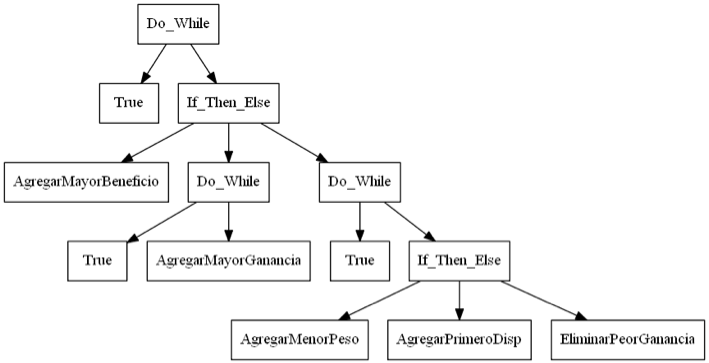
\includegraphics[width=13cm]{images/cap6/AIKPDC2.png}
    \captionof{figure}{Mejor algoritmo del experimento 1 por menor ERP (Elaboración propia, 2015)}\label{fig:AIKPDC2}
\endgroup

%Podría agregar algo respecto a que grupo pertenecen las mejores

Algunas estructuras algorítmicas descubiertas por la PG parecen ser más eficientes que otras en la determinación de la mejor solución para la mochila. Específicamente, es posible apreciar en las figuras que representan los árboles sintácticos que el terminal más utilizado es el de “AgregarMayorGanancia”. Este terminal, en varias ocasiones va acompañado de un ciclo \textit{“while”}, lo que permite llenar la mochila siguiendo el criterio de llenado de este terminal. El terminal que elimina ítems de la mochila que más aparece es “EliminarPeorGanancia”, el cual es utilizado por los algoritmos para eliminar algunos de los elementos y, posteriormente, utilizar otro terminal para llenar el espacio restante. El terminal que aparece posterior al de “EliminarPeorGanancia” es el de “AgregarMenosPeso”, que sirve para agregar un refinamiento al criterio entregado por el terminal de “AgregarMayorGanancia”. Las estructuras siguen la misma lógica de los algoritmos goloso que en algunos casos presenta un refinamiento por medio de la eliminación de algunos ítems para posteriormente realizar un nuevo ingreso de éstos bajo otro criterio.

\subsection{Construcciones inocuas}

Algunos de los algoritmos generados por los métodos utilizados, poseen una estructura inútil o ineficiente. Esto ocurre porque una estructura que deja la mochila vacía, cumple con el criterio de suficiencia, ya que es una posible solución, aunque la calidad de ésta no es buena. Estas soluciones son parte del proceso evolutivo y la forma en que éste las deja de considerar el por medio de la función de evaluación. Algunas de las estructuras generadas son las siguientes:
\begin{itemize}
	\item IfThen(Agregar, Eliminar): esta estructura agrega un elemento y luego lo elimina.
	\item Do\_While(Agregar, Eliminar), Do\_While(True, Eliminar), Do\_While(Eliminar, Eliminar): en estas estructuras ocurre un efecto similar al de la estructura anterior, pero un máximo de tres veces, debido a que el ciclo \textit{“while”} fue implementado con un criterio de término si no genera cambios en la función de evaluación en tres iteraciones.
	\item Not(Eliminar): retorna verdadero, pero no realiza ningún cambio en la mochila.
\end{itemize}

\section{Resultados PVV}

\subsection{Resultados del proceso evolutivo}

Para el problema del vendedor viajero, la GAA converge de forma sistemática para las diversas ejecuciones realizadas. El efecto es similar al ocurrido en el PM-01 y a otros trabajos de la literatura, donde se produce una convergencia en los resultados para ambos experimentos. La Figura \ref{fig:convergencia_exp3} y la Figura \ref{fig:convergencia_exp4} muestran las ejecuciones realizadas por los experimentos 3 y 4 de acuerdo al \textit{fitness} a lo largo de las generaciones. En los gráficos, cada línea corresponde al mejor algoritmo de cada ejecución del programa. En estas figuras es posible apreciar la rápida convergencia de las ejecuciones y que el \textit{fitness} de cada una de éstas converge a un valor similar.

\begingroup
    \centering
    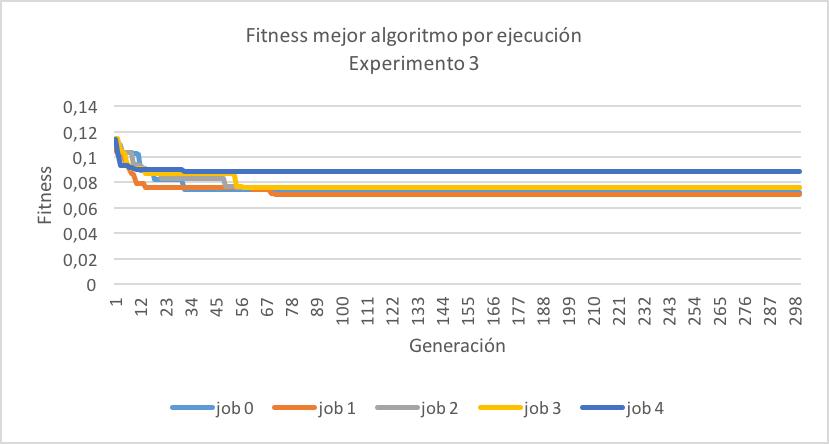
\includegraphics[width=13cm]{images/cap6/convergencia_exp3.png}
    \captionof{figure}{Fitness del mejor algoritmo de cada ejecución por generación para el experimento 3 (Elaboración propia, 2015)}\label{fig:convergencia_exp3}
\endgroup

\begingroup
    \centering
    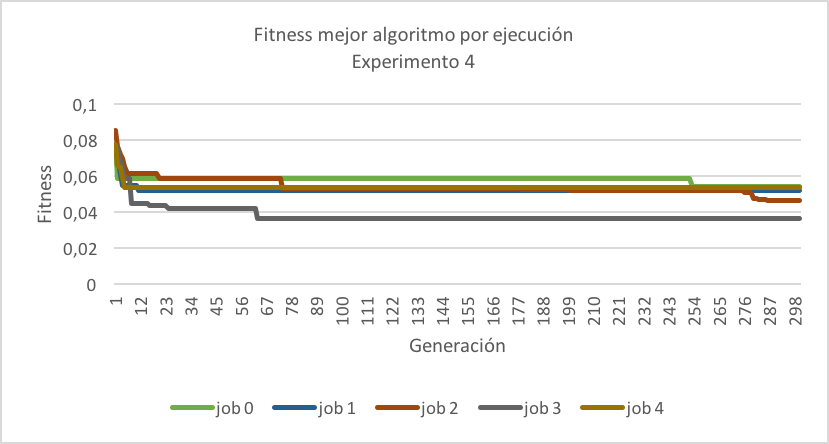
\includegraphics[width=13cm]{images/cap6/convergencia_exp4.png}
    \captionof{figure}{Fitness del mejor algoritmo de cada ejecución por generación ppara el experimento 4 (Elaboración propia, 2015)}\label{fig:convergencia_exp4}
\endgroup

Existe una gran variedad en relación a la calidad de los algoritmos obtenidos. La distribución de los algoritmos por medio de su calidad en el proceso evolutivo a través de las generaciones, es presentada en las Figuras \ref{fig:box_whisker_exp3} y \ref{fig:box_whisker_exp4}. Estas figuras presentan el \textit{fitness} de los algoritmos obtenidos en el proceso evolutivo del experimento 3 y el experimento 4, mediante el uso de un gráfico de \textit{Box and Whisker}. Al igual que para el PM-01, en estas Figuras solo son representadas algunas generaciones (0, 25, 50, 75, …, 299), para así poder apreciar la distribución de los algoritmos, debido a su extensa cantidad de algoritmos generados. Al igual que para el PM-01, es posible inferir que al inicio del proceso evolutivo la mayor cantidad de los individuos posee los peores valores de \textit{fitness}, para el experimento 3 en la generación 0 los cuatro cuartiles se encuentran en un rango de $4.000$ a $4.500$, ya en la generación 25 aparecen individuos con un \textit{fitness} bajo, lo que posiciona los cuartiles en un rango de \textit{fitness} de $0$ a $4.000$ y, posteriormente al avanzar las generaciones se converge a menores valores para la población. Para el experimento 2 se aprecia que en la generación 0 se inicia con un rango de \textit{fitness} de $0$ a $7.000$, donde la mitad de los algoritmos tiene un \textit{fitness} menor a $2.000$, a medida que avanzan las generaciones, esta distribución tiende a mejores valores, los que por la escala generada para mostrar la primera generación no logran apreciarse graficamente, pero éstos oscilan en un rango entre $0$ y $1$, es decir, la “caja” se encuentra dentro del rango mencionado. En general, es posible apreciar que existen varios \textit{outliers} en ambos gráficos, los que se encuentran distribuidos en la parte superior de las “cajas”. En particular el gráfico presentado en la Figura \ref{fig:box_whisker_exp4}, desde la generación 25 en adelante solo es posible apreciar los \textit{outliers}, esto se debe a que las parsimonias aplicadas a este problema empeoran de forma considerable los valores del \textit{fitness}. En ambos gráficos el \textit{fitness} promedio converge a valores menores que oscilan entre $500$ y $1.000$, mientras que la media tiende a $0$ o valores muy pequeños. De esto último, se desprende que los algoritmos tienden a “eliminar” los valores de las parsimonias para mejorar su valor de \textit{fitness} a medida que avanzan las generaciones. La distribución sigue una tendencia de mejora en los resultados de la función de evaluación que es lo esperado. Este efecto ocurre en todas las ejecuciones y aunque la distribución no es igual para todos los casos, sigue una tendencia similar a las presentadas en las figuras descritas anteriormente. La tendencia de los algoritmos puede ser inferida de la Tabla \ref{tab:resumen_exp3} y \ref{tab:resumen_exp4}, donde es posible apreciar que los algoritmos presentan similitudes en sus valores máximos, mínimos y promedio. Dada la cantidad de algoritmos generados, se selecciona para el proceso de evaluación, solo al mejor individuo de cada una de las ejecuciones por experimento. Como resultado, son evaluados 10 algoritmos, siendo cinco los extraídos del experimento 3 y los otros cinco del experimento 4. 

\begingroup
    \centering
    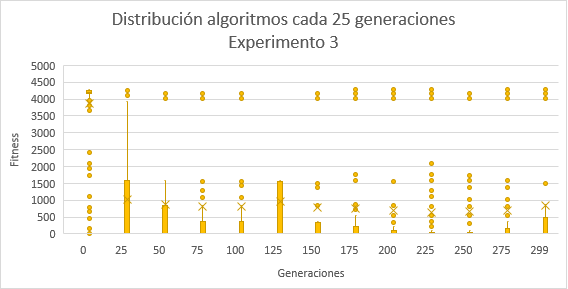
\includegraphics[width=14cm]{images/cap6/box_whisker_exp3.png}
    \captionof{figure}{Distribución de los algoritmos experimento 3 (Elaboración propia, 2015)}\label{fig:box_whisker_exp3}
\endgroup

\begingroup
    \centering
    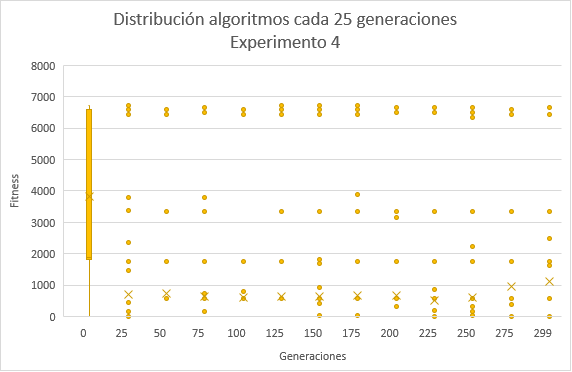
\includegraphics[width=14cm]{images/cap6/box_whisker_exp4.png}
    \captionof{figure}{Distribución de los algoritmos experimento 4 (Elaboración propia, 2015)}\label{fig:box_whisker_exp4}
\endgroup

\begin{table}[ht]
\caption{Datos generales de los algoritmos obtenidos en el experimento 3}\label{tab:resumen_exp3}
\small
\centering
\begin{center}
\rowcolors{2}{gray!25}{white}
\begin{tabular}{c|ccc|ccc|ccc}
\hline
{\textbf{}} & \multicolumn{3}{c}{{\textbf{Fitness}}} & \multicolumn{3}{c}{{\textbf{Nº Nodos}}} & \multicolumn{3}{c}{{\textbf{Altura}}} \\ \hline
{\textbf{Nombre}} & \textbf{Peor} &	\textbf{Prom.} & \textbf{Mejor} & \textbf{Min.} & \textbf{Prom.} & \textbf{Máximo} & \textbf{Min.} & \textbf{Prom.} & \textbf{Máximo} \\ \hline
ejec. 0 & 6731,6667 & 678,8823 & 0,0538 & 2 & 6,4742 & 120 & 2 & 3,1448 & 10 \\
ejec. 1 & 6731,0667 & 1072,3096 & 0,0520 & 2 & 8,7007 & 131 & 2 & 4,1905 & 10 \\
ejec. 2 & 6734,2000 & 867,7404 & 0,0461 & 2 & 9,3059 & 140 & 2 & 4,6702 & 10 \\
ejec. 3 & 6732,2667 & 739,3558 & 0,0364 & 2 & 7,9342 & 126 & 2 & 3,6788 & 10 \\
ejec. 4 & 6733,4000 & 1107,9228 & 0,0533 & 2 & 8,6260 & 133 & 2 & 3,3546 & 9 \\
\hline
\end{tabular}
\end{center}
\caption*{(Elaboración propia, 2015)}
\end{table}

\begin{table}[ht]
\caption{Datos generales de los algoritmos obtenidos en el experimento 4}\label{tab:resumen_exp4}
\small
\centering
\begin{center}
\rowcolors{2}{gray!25}{white}
\begin{tabular}{c|ccc|ccc|ccc}
\hline
{\textbf{}} & \multicolumn{3}{c}{{\textbf{Fitness}}} & \multicolumn{3}{c}{{\textbf{Nº Nodos}}} & \multicolumn{3}{c}{{\textbf{Altura}}} \\ \hline
{\textbf{Nombre}} & \textbf{Peor} &	\textbf{Prom.} & \textbf{Mejor} & \textbf{Min.} & \textbf{Prom.} & \textbf{Máximo} & \textbf{Min.} & \textbf{Prom.} & \textbf{Máximo} \\ \hline
ejec. 0 & 4300,1444 & 849,5119 & 0,0724 & 2 & 11,5701 & 117 & 2 & 5,0646 & 10 \\
ejec. 1 & 4299,8778 & 870,1784 & 0,0708 & 2 & 12,2544 & 104 & 2 & 6,4230 & 10 \\
ejec. 2 & 4303,7444 & 1168,2259 & 0,0758 & 2 & 10,5527 & 146 & 2 & 4,5922 & 10 \\
ejec. 3 & 4301,3444 & 336,8097 & 0,0762 & 2 & 12,6993 & 127 & 2 & 6,0875 & 10 \\
ejec. 4 & 4301,2778 & 1422,5640 & 0,0889 & 2 & 7,0219 & 132 & 2 & 3,4251 & 10 \\
\hline
\end{tabular}
\end{center}
\caption*{(Elaboración propia, 2015)}
\end{table}

No existe una gran variación en la calidad de la GAA para los distintos algoritmos obtenidos durante el proceso evolutivo para el mismo conjunto de instancias. En las tablas \ref{tab:resumen_exp3} y \ref{tab:resumen_exp4} aparecen datos del mejor, peor y promedio del \textit{fitness} de todos los algoritmos generados utilizando alguno de los grupos de instancias clasificados en el sub-capítulo \ref{cap:sel_casos_adapt_pvv}. En relación a la Tabla \ref{tab:resumen_exp3}, es posible apreciar que el resultado tanto del mejor y el peor \textit{fitness} de los algoritmos tiende a valores similares, mientras que el promedio presenta una mayor variación, lo que se debe a la escala de los números obtenidos por la penalización en la función de evaluación (véase \ref{cap:func_eval_pvv}), donde la aparición de uno más o uno menos de los algoritmos con peor \textit{fitness} influye considerablemente. Para la Tabla \ref{tab:resumen_exp4} se ve que ocurre un efecto similar. Finalmente, los resultados que se obtienen en cada uno de los grupos al ser comparados entre experimentos, presentan una variación en la que los algoritmos del experimento 3 obtienen mejores resultados. Esta variación ocurre por que en el experimento 4 se generan algoritmos en distintas poblaciones con distintos criterios de evaluación (islas), lo que conlleva a una mayor variabilidad que la presentada en el experimento 3.

La variación de los algoritmos obtenidos en la GAA está relacionada con la estructura  que posee el árbol sintáctico obtenido durante el proceso evolutivo. Un efecto similar al presentado para los experimentos relacionados al PM-01, ocurre en las tablas \ref{tab:resumen_exp3} y \ref{tab:resumen_exp4}, donde aparecen datos del máximo, mínimo y promedio del número de nodos y la altura. Con respecto al número de nodos, existe variación en los algoritmos que alcanza valores máximos sobre 100, mientras que el promedio es siempre menor a 15, cuyo valor fue determinado como máximo para no interferir en la calidad de los algoritmos (factor de legibilidad, véase \ref{cap:func_eval_pvv}). En relación a la altura de los árboles que representan a los algoritmos, se ve que también existe variación en el promedio. Esto se relaciona directamente con el número de nodos máximo permitido, ya que algunos de estos nodos representan funciones, las que solo tienen permitido un número determinado de hijos.

La calidad de los algoritmos obtenidos mediante el proceso evolutivo no tiene relación con el tiempo que demora el proceso evolutivo ni la generación en la que el o los mejores algoritmos aparecen dentro de la ejecución de este proceso. En las tablas \ref{tab:mejores_pvv_exp3} y \ref{tab:mejores_pvv_exp4}, es posible apreciar el tiempo de evolución de cada una de las ejecuciones y la generación en la que aparece el mejor individuo de ésta. En estas tablas, además, es posible notar que existe variación tanto en el tiempo de cada una de las ejecuciones del proceso evolutivo y en la generación en la que el mejor individuo aparece. El nombre de los algoritmos posee la siguiente forma: Algoritmo - Experimento (Tradicional \textbf{(N)} o co-evolución utilizando método de islas \textbf{(I)}) - Problema - Correlativo de 1 a 5. Un ejemplo de esto último es ANTSP1, que se lee como Algoritmo (A) del experimento tradicional (N) para el problema del vendedor viajero (TSP) obtenido en la ejecución 1.

El tamaño de los árboles que componen los algoritmos obedece al rango de tamaño predefinido en la función de legibilidad que se encuentra dentro de la función de evaluación (\textit{fitness}). En las tablas \ref{tab:mejores_pvv_exp3} y \ref{tab:mejores_pvv_exp4} se muestra que no existe una convergencia hacia árboles de similares dimensiones. Como se observa en estas tablas, los árboles seleccionados varían entre 8 y 15 nodos con una altura entre 4 y 8 para el experimento 3, y entre 3 y 15 nodos, con una altura entre 2 y 6 para el experimento 4.

\begin{table}[ht]
\caption{Datos generales del mejor algoritmo de cada experimento del experimento 3}\label{tab:mejores_pvv_exp3}
\small
\centering
\begin{center}
\rowcolors{2}{gray!25}{white}
\begin{tabular}{cccccc}
{\textbf{{Nombre}}} & {\textbf{{Fitness}}} & {\textbf{\begin{tabular}[c]{@{}c@{}}Nº de \\nodos\end{tabular}}} & {\textbf{{Altura}}} & {\textbf{\begin{tabular}[c]{@{}c@{}}Ejecución en la \\que aparece\end{tabular}}} & {\textbf{\begin{tabular}[c]{@{}c@{}}Tiempo \\(horas)\end{tabular}}}\\ \hline
ANTSP1 & 0,0528 & 13 & 6 & 140 & 24,2040 \\
ANTSP2 & 0,0511 & 15 & 8 & 70 & 23,8845 \\
ANTSP3 & 0,0535 & 15 & 6 & 51 & 19,1857 \\
ANTSP4 & 0,0539 & 15 & 7 & 56 & 24,0360 \\
ANTSP5 & 0,0614 & 8 & 4 & 29 & 14,1123 \\
\hline
\end{tabular}
\end{center}
\caption*{(Elaboración propia, 2015)}
\end{table}


\begin{table}[ht]
\caption{Datos generales del mejor algoritmo de cada experimento del experimento 4}\label{tab:mejores_pvv_exp4}
\small
\centering
\begin{center}
\rowcolors{2}{gray!25}{white}
\begin{tabular}{ccccccc}
{\textbf{{Nombre}}} & {\textbf{{Fitness}}} & {\textbf{\begin{tabular}[c]{@{}c@{}}Nº de \\nodos\end{tabular}}} & {\textbf{{Altura}}} & {\textbf{\begin{tabular}[c]{@{}c@{}}Ejecución en la \\que aparece\end{tabular}}} & {\textbf{\begin{tabular}[c]{@{}c@{}}Isla en la \\que aparece\end{tabular}}} & {\textbf{\begin{tabular}[c]{@{}c@{}}Tiempo \\(horas)\end{tabular}}}\\ \hline
AITSP1 & 0,0803 & 3 & 2 & 2 & 0 & 16,6950 \\
AITSP2 & 0,0558 & 13 & 7 & 271 & 2 & 13,0391 \\
AITSP3 & 0,0621 & 11 & 5 & 182 & 3 & 13,9234 \\
AITSP4 & 0,0544 & 9 & 4 & 62 y 54 & 1 y 3 & 10,8758 \\
AITSP5 & 0,0620 & 15 & 5 & 262 & 2 & 14,9751 \\
\hline
\end{tabular}
\end{center}
\caption*{(Elaboración propia, 2015)}
\end{table}

Las parsimonias utilizadas en los algoritmos no afectan el proceso evolutivo. En los experimentos 3 y 4 se agregaron elementos a la función de evaluación o \textit{fitness} que consideraban una penalización para características propias del problema que generen infactibilidades. Estos elementos empeoran de forma exponencial los valores de la función de evaluación al inicio del proceso evolutivo, y a medida que las generaciones avanzan, estos valores disminuyen llegando a cero. En la Tabla \ref{tab:parsimonias} se puede ver que los elementos de la parsimonia se hacen 0 para todos los mejores algoritmos obtenidos en ambos experimentos. Estos resultados son esperables, ya que las parsimonias afectan en mayor medida (mayor escala) a la función de evaluación, y los elementos que la componen no presentan mayor dificultad, debido a que principalmente se ven afectadas en caso de que los circuitos no estén completos, es decir, se produzca una solución infactible.

\begin{table}[hbtp!]
\caption{Elementos de la parsimonia para los mejores algoritmos de cada experimento.}\label{tab:parsimonias}
\small
\centering
\begin{center}
\begin{tabular}{ccccccc}
{\textbf{Experimento}} & {\textbf{Nombre}} & {\textbf{$ERP$}} & {\textbf{$leg$}} & {\textbf{$PPA$}} & {\textbf{$ERC$}} & {\textbf{$Fitness$}} \\ \hline
Experimento 3		& 	\begin{tabular}[c]{@{}c@{}} ANTSP1 \\ ANTSP2 \\ ANTSP3 \\ ANTSP4 \\ ANTSP5  \end{tabular} &
						\begin{tabular}[c]{@{}c@{}} 0,0528 \\ 0,0511 \\ 0,0535 \\ 0,0539 \\ 0,0614  \end{tabular} &
						\begin{tabular}[c]{@{}c@{}}  0 	   \\ 0 	 \\ 0 	   \\ 0 	 \\ 0 		\end{tabular} &
						\begin{tabular}[c]{@{}c@{}} 4296,6111 \\ 4296,6111 \\ 4296,6111 \\ 4296,6111 \\ 4296,6111 \end{tabular} &
						\begin{tabular}[c]{@{}c@{}}  0 	   \\ 0 	 \\ 0 	   \\ 0 	 \\ 0 		\end{tabular} &
						\begin{tabular}[c]{@{}c@{}} 0,0528 \\ 0,0511 \\ 0,0535 \\ 0,0539 \\ 0,0614  \end{tabular} \\ \hline
Experimento 4		& 	\begin{tabular}[c]{@{}c@{}} AITSP1 \\ AITSP2 \\ AITSP3 \\ AITSP4 \\ AITSP5  \end{tabular} &
						\begin{tabular}[c]{@{}c@{}} 0,0803 \\ 0,0558 \\ 0,0621 \\ 0,0544 \\ 0,0620  \end{tabular} &
						\begin{tabular}[c]{@{}c@{}}  0 	   \\ 0 	 \\ 0 	   \\ 0 	 \\ 0 		\end{tabular} &
						\begin{tabular}[c]{@{}c@{}} 4296,6111 \\ 4296,6111 \\ 4296,6111 \\ 4296,6111 \\ 4296,6111 \end{tabular} &
						\begin{tabular}[c]{@{}c@{}}  0 	   \\ 0 	 \\ 0 	   \\ 0 	 \\ 0 		\end{tabular} &
						\begin{tabular}[c]{@{}c@{}} 0,0803 \\ 0,0558 \\ 0,0621 \\ 0,0544 \\ 0,0620  \end{tabular} \\
\hline
\end{tabular}
\end{center}
\caption*{(Elaboración propia, 2015)}
\end{table}

Los algoritmos generados a partir del proceso evolutivo utilizando el grupo de instancias con un menor coeficiente de correlación obtienen mejores resultados. Para la clasificación de instancias a utilizar por cada una de las islas es utilizado su coeficiente de correlación. En la Tabla \ref{tab:mejores_islas_pvv} se presentan los resultados de los mejores algoritmos de cada isla por ejecución. En esta Tabla se puede ver los resultados del ERP que obtuvo cada uno de éstos y el \textit{fitness} con el que finalmente fueron evaluados durante el proceso evolutivo. Considerando los resultados obtenidos en las ejecuciones de los experimentos donde las islas 0 y 2 utilizan el grupo de instancias 2 y las islas 1 y 3 utilizan el grupo de instancias 1, es posible apreciar que existe una diferencia en la calidad de los resultados de los algoritmos en el proceso evolutivo, que en algunas ejecuciones es menor a un 2\% de ERP al comparar las islas 1 y 3 con las otras islas. Por otra parte, los resultados para las islas 0 y 3, que poseen igual función de evaluación por HITS (cantidad de soluciones óptimas obtenidas), presentan una gran variación entre el ERP y el \textit{fitness}, mientras que en las islas 1 y 2 con función de evaluación por medio de su ERP, obtienen resultados similares. Este efecto es similar al presentado en los resultados del PM-01, donde la función de evaluación, cuando es relacionada a los HITS para obtener el valor del \textit{fitness}, presentan una calidad similar tanto si su ERP es bueno como si no lo es.

\begin{table}[hbtp!]
\caption{Resumen del fitness promedio y ERP de cada isla por ejecución del experimento 4}\label{tab:mejores_islas_pvv}
\small
\centering
\begin{center}
\rowcolors{2}{gray!25}{white}
\begin{tabular}{c|cc|cc|cc|cc}
{\textbf{}} & \multicolumn{2}{c|}{{\textbf{Isla 0}}} & \multicolumn{2}{c|}{{\textbf{Isla 1}}} & \multicolumn{2}{c|}{{\textbf{Isla 2}}} & \multicolumn{2}{c}{{\textbf{Isla 3}}}\\ \hline
{\textbf{Nombre}} & {\textbf{ERP}} & {\textbf{Fitness}} & {\textbf{ERP}} & {\textbf{Fitness}} & {\textbf{ERP}} & {\textbf{Fitness}} & {\textbf{ERP}} & {\textbf{Fitness}} \\ \hline
ejec. 0 & 0,0876 & 0,6667 & 0,0538 & 0,0538 & 0,0638 & 0,0638 & 0,0687 & 0,4444 \\
ejec. 1 & 0,0768 & 0,6667 & 0,0520 & 0,0520 & 0,0540 & 0,0540 & 0,0548 & 0,4444 \\
ejec. 2 & 0,0586 & 0,4444 & 0,0461 & 0,0461 & 0,0545 & 0,0545 & 0,0523 & 0,3333 \\
ejec. 3 & 0,0686 & 0,5556 & 0,0364 & 0,0364 & 0,0521 & 0,0521 & 0,0364 & 0,2222 \\
ejec. 4 & 0,0876 & 0,6667 & 0,0533 & 0,0533 & 0,0582 & 0,0582 & 0,0636 & 0,4444 \\
\hline
\end{tabular}
\end{center}
\caption*{(Elaboración propia, 2015)}
\end{table}

\subsection{Resultados de la evaluación}

Los algoritmos seleccionados para el proceso de evaluación empeoran al comparar los resultados obtenidos para los grupos de instancias de evolución en comparación a los de evaluación. La Figura \ref{fig:evol_vs_eval_exp3_4} muestra los resultados de la comparación entre los resultados de la evolución y evaluación para los experimentos 3 y 4.

\begingroup
    \centering
    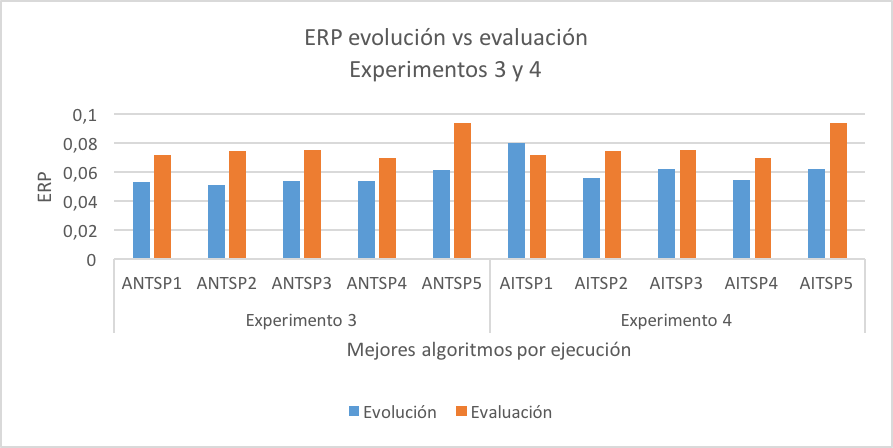
\includegraphics[width=14cm]{images/cap6/evol_vs_eval_exp3_4.png}
    \captionof{figure}{ERP de los resultados obtenidos en la evaluación del grupo de instancias de evolución en comparación al grupo de evaluación (Elaboración propia, 2015)}\label{fig:evol_vs_eval_exp3_4}
\endgroup

Los algoritmos producidos son muy rápidos para resolver los problemas del vendedor viajero. En la Tabla \ref{tab:evol_vs_eval_tiempos_exp3_4} se muestra el tiempo que le toma al mejor algoritmo de cada ejecución resolver las instancias de evaluación para el experimento 3 y 4. El tiempo empleado por los algoritmos del experimento 3 es en promedio 6 minutos y medio, alcanzando menos de 5 minutos el más rápido y casi 11 minutos el más lento de ellos. Los algoritmos más rápidos resuelven en seis segundos aproximados cada instancia, mientras que los más lentos las resuelven en poco más de 12 segundos. Para los algoritmos generados en el experimento 4, se tienen tiempos similares. Estos resultados son esperables, ya que los terminales son acciones con complejidad polinomial y de las funciones sólo el ciclo \textit{while} puede aumentar la complejidad de los algoritmos producidos, sin embargo, este posee una restricción de termino en caso de que en más de tres iteraciones no se produzca algún cambio en el valor de la función de evaluación.
%Agregar el tamaño de las instancias de evaluación.

\begin{table}[hbtp!]
\caption{Tiempo que demoran los mejores algoritmos para resolver las instancias de evaluación}\label{tab:evol_vs_eval_tiempos_exp3_4}
\small
\centering
\begin{center}
\rowcolors{2}{gray!25}{white}
\begin{tabular}{cc|cc}
\multicolumn{2}{c|}{{\textbf{Experimento 3}}} & \multicolumn{2}{c}{{\textbf{Experimento 4}}} \\ \hline
{\textbf{Nombre}} & {\textbf{Tiempo (min)}} & {\textbf{Nombre}} & {\textbf{Tiempo (min)}} \\ \hline
ANTSP1 & 5,7883 & AITSP1 & 5,7883 \\
ANTSP2 & 4,8759 & AITSP2 & 4,8759 \\
ANTSP3 & 5,0715 & AITSP3 & 5,0715 \\
ANTSP4 & 10,5594 & AITSP4 & 10,5594 \\
ANTSP5 & 5,9571 & AITSP5 & 5,9571 \\
\hline
\end{tabular}
\end{center}
\caption*{(Elaboración propia, 2015)}
\end{table}

Los algoritmos obtenidos mediante el proceso co-evolutivo utilizando el método de islas tienen un desempeño computacional similar a los algoritmos obtenidos mediante el proceso tradicional. Los algoritmos obtenidos durante el proceso evolutivo en ambos experimentos para el PVV no logran obtener soluciones óptimas, por lo que no es posible obtener los mejores de acuerdo a la cantidad de soluciones óptimas. Es por esto que sólo se utiliza el criterio de menor ERP para seleccionar a los mejores. En la Tabla \ref{tab:mejores_exp_erp_pvv} se muestran los resultados del mejor algoritmo obtenido para cada experimento de acuerdo a su menor ERP en el grupo de evaluación. En esta Tabla se presentan los indicadores de cada algoritmo y el error relativo que se obtuvo al evaluar los algoritmos con el mismo conjunto de instancias de evaluación y la cantidad de soluciones óptimas que encuentra. 
Tal como se observa, el error relativo promedio de los algoritmos del primer experimento es similar al del segundo experimento. Los resultados obtenidos por ambos experimentos siguen una distribución normal, así lo muestra el \textit{test de Shapiro-Wilk}. En consecuencia,  el \textit{test} de ANOVA que proporciona bajo un 95\% de confiabilidad que no existe diferencia significativa en los datos obtenidos, por lo que no es posible rechazar la hipótesis nula. El resultado contrasta descubrimientos realizados por otros autores para algoritmos genéticos, lo que puede ser inferido puesto que algunos de los resultados obtenidos utilizando el método de la PG con co-evolución muestran una mejora en la calidad de los algoritmos, la que es estadísticamente despreciable.

\begin{table}[hbtp!]
\caption{Mejores individuos por menor ERP en grupo de evaluación}\label{tab:mejores_exp_erp_pvv}
\small
\centering
\begin{center}
\begin{tabular}{cc|ccc|ccc}
\multicolumn{2}{c}{{\textbf{ }}} & \multicolumn{3}{|c|}{{\textbf{Error Relativo}}} & \multicolumn{3}{c}{{\textbf{ }}} \\
{\textbf{Exp.}} & {\textbf{Nombre}} & {\textbf{Peor}} & {\textbf{Prom.}} & {\textbf{Mejor}} & {\textbf{Soluciones}} & {\textbf{Nodos}} & {\textbf{Altura}}\\ \hline
Tradicional & ANTSP4 & 0,1094 & 0,0693 & 0,0114 & 0 & 15 & 7 \\
Islas & AITSP2 & 0,1144 & 0,0672 & 0,0229 & 0 & 13 & 7 \\
\hline
\end{tabular}
\end{center}
\caption*{(Elaboración propia, 2015)}
\end{table}


\subsection{Estructuras de los algoritmos generados}

En esta sección se presenta una figura que muestra el árbol sintáctico del algoritmo junto a una breve explicación de cómo funciona. Los algoritmos descritos en esta sección incluyen los algoritmos señalados en la Tabla \ref{tab:mejores_exp_erp_pvv}. Estos algoritmos son $ANTSP4$ para el experimento 3 y $AITSP2$ para el experimento 4, que fueron seleccionados por obtener el menor ERP al ser evaluados en las instancias de evaluación.

\subsubsection{ANTSP4}

El $ANTSP4$ es el mejor algoritmo obtenido en el experimento 3. En la Figura \ref{fig:ANTSP4} se puede ver el algoritmo por medio de su árbol sintáctico. Este algoritmo posee 15 nodos y una altura de 7, compuesto de 8 terminales y 7 funciones. Este algoritmo sigue una lógica puramente constructiva, donde utilizando distintos criterios tiene por objetivo sólo completar el circuito.

Los pasos a realizar por este algoritmo inician con el ciclo \textit{“while”} con la condición de intentar agregar el mejor vecino. A continuación, pregunta si es posible agregar el mejor vecino y nuevamente aparece la estructura que realiza la misma pregunta. Si ambas son posibles, se intenta agregar una ciudad que genere el menor arco. Posteriormente, si es posible agregar el elemento más cercano al centro, se prosigue a agregar la ciudad que genere el menor arco. Más adelante, se entra a un nuevo ciclo que itera agregando el mejor vecino y la ciudad que genere el menor arco hasta completar el circuito. Finalmente, el circuito creado por el algoritmo es sometido a la heurística \textit{2-opt} para intentar mejorar el resultado.

\begingroup
    \centering
    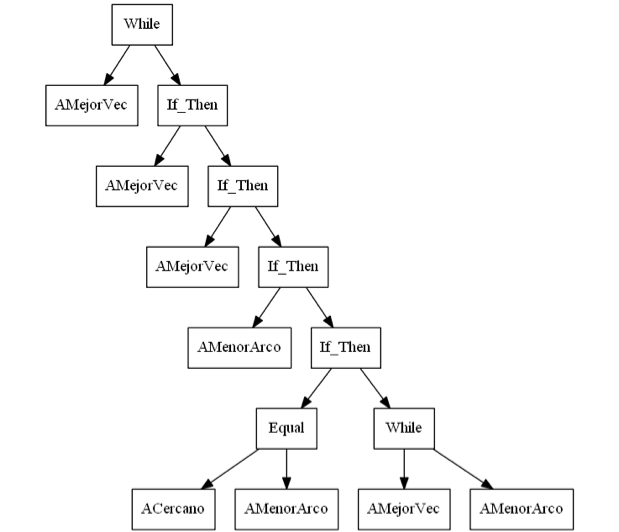
\includegraphics[width=13cm]{images/cap6/ANTSP4.png}
    \captionof{figure}{Mejor algoritmo del experimento 3 (Elaboración propia, 2015)}\label{fig:ANTSP4}
\endgroup

\subsubsection{AITSP2}

El $AITSP2$ es el mejor algoritmo obtenido en el experimento 4. En la Figura \ref{fig:AITSP2} se puede ver el algoritmo por medio de su árbol sintáctico. Este algoritmo posee 13 nodos y una altura de 7, se encuentra compuesto de 6 terminales y 7 funciones. Este algoritmo también sigue una lógica puramente constructiva, donde utilizando distintos criterios tiene por objetivo sólo completar el circuito.
La estructura de este árbol es similar a la obtenida por el mejor algoritmo del experimento 3. En esta estructura se inicia con la adición al circuito del elemento más cercano al centro, para luego agregar la ciudad que genere el menor arco. A continuación, se inicia un ciclo donde si es posible agregar la ciudad que genere el menor arco, se procede a agregar el más cercano al centro. Si esto es posible, se itera agregando la ciudad que genere el menor arco y el mejor vecino hasta completar el circuito. Finalmente, el circuito creado por el algoritmo es sometido a la heurística \textit{2-opt} para intentar mejorar el resultado.

\begingroup
    \centering
    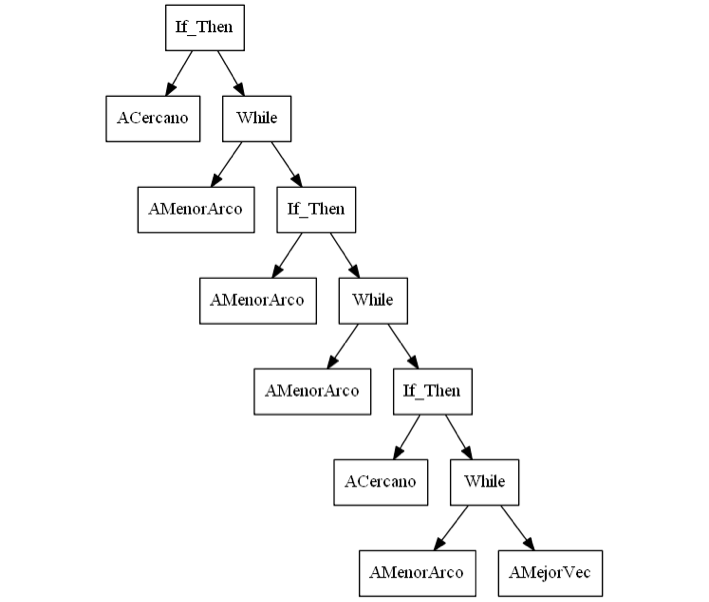
\includegraphics[width=14cm]{images/cap6/AITSP2.png}
    \captionof{figure}{Mejor algoritmo del experimento 4 (Elaboración propia, 2015)}\label{fig:AITSP2}
\endgroup

Algunas estructuras algorítmicas descubiertas por la PG parecen ser más eficientes que otras en la determinación de la mejor solución para el PVV. Específicamente, es posible apreciar en las figuras que representan los árboles sintácticos que los terminales más utilizados son los de “AMenorArco” y “AMejorVecino”. Éstos permiten armar el circuito agregando las ciudades que aumenten en menor medida el costo del circuito con dos criterios. Los criterios son agregar el de menor costo al final y el de agregar una ciudad en cualquier parte del circuito que aumente de menor medida el costo, para “AMenorArco” y “AMejorVecino” respectivamente. El otro terminal que aparece es el de “ACercano”, que agrega al final del circuito la ciudad más cercana al centro. Finalmente, se opera la heurística de optimización \textit{2-opt}, lo que finalmente produce una mejora sustancial sobre las soluciones. En conclusión, los algoritmos generados buscan la producción de un buen circuito para ser optimizado por la heurística \textit{2-opt}.

\subsection{Construcciones inocuas}

Los algoritmos producidos por los experimentos 3 y 4 tienen un efecto similar en algunos de los árboles producidos en los otros experimentos. Algunos de estos efectos son los producidos por las estructuras inútiles. Estas estructuras operan sobre las ciudades del circuito, pero finalmente el resultado es un circuito vacío. Estas soluciones son parte del proceso evolutivo y la forma en que éste las deja de considerar el por medio de la función de evaluación. Algunas de las estructuras generadas son las siguientes:

\begin{itemize}
	\item IfThen(Agregar, Eliminar): esta estructura agrega una ciudad y luego la elimina.
	\item Do\_While(Agregar, Eliminar), Do\_While(True, Eliminar), Do\_While(Eliminar, Eliminar): en estas estructuras se agregan y eliminan elementos de forma iterativa, resultando en que la salida es el circuito vacío.
	\item Not(Eliminar): retorna verdadero, pero no realiza ningún cambio en el circuito.
	\item Las estructuras son similares, ya que los terminales de forma general agregan o eliminan elementos a la solución.
\end{itemize}
